\documentclass[a4paper,12pt]{article}
\usepackage{fancyvrb}
\usepackage{amsfonts}
\usepackage{graphicx}
\usepackage{tabularx}
% \usepackage{color}
\usepackage{xcolor}
\usepackage{psfrag}
\usepackage[hyphens]{url}
% \usepackage{vmargin}
\usepackage{cite}
\usepackage{caption2}
\usepackage{hyperref}
\usepackage{makeidx}
\usepackage[fleqn]{amsmath}
\renewcommand{\captionlabeldelim}{.}
\def\thesection{\arabic{section}}
\renewcommand{\thefigure}{\arabic{figure}}
\renewcommand{\thetable}{\arabic{table}}
\newcommand{\hl}{\noalign{\vskip3pt}\hline\noalign{\vskip3pt}}
\newcommand{\hrf}{\hrulefill}
\newcommand{\tc}[1]{\textcolor{black}{#1}}
\newcommand{\dc}[1]{\textcolor{green}{#1}}
% \usepackage[none]{hyphenat}
\newcommand{\rep}[3][1]
{
  \psfrag{#2}[c][c][#1]{#3}
}
\newcommand{\x}[1]{\texttt{#1}}
\newcommand{\sfv}{$\Lambda$V}

\DeclareMathOperator*{\Ex}{\mathbb{E}}
\newcommand{\Var}{\mathrm{Var}}

% \setpapersize{A4}
% \hypersetup{colorlinks=true,linkcolor=blue,urlcolor=red,linkbordercolor=000}
\hypersetup{colorlinks=true,linkcolor=blue,urlcolor=orange}
\renewcommand{\baselinestretch}{1.}
\makeindex
\begin{document}
\sloppy
\begin{center}
\thispagestyle{empty}
\vfill\vfill
% \rule{\linewidth}{0.02cm}\\
{\Huge \textbf{ P~h~y~M~L~~--~~M~a~n~u~a~l}}
\vspace{-0.4cm}\\
% \rule{\linewidth}{0.02cm}\\
\vfill
{\huge Version 3.0 \\
\today
\vfill
\normalsize
\href{https://github.com/stephaneguindon/phyml}{https://github.com/stephaneguindon/phyml}\\
\vspace{0.4cm}
\href{http://www.atgc-montpellier.fr/phyml}{http://www.atgc-montpellier.fr/phyml}}
\end{center}
\clearpage
\tableofcontents
\clearpage

{\par
\small
\noindent
\copyright Copyright 1999 - 2008 by PhyML Development Team.\\
\noindent The software PhyML is provided ``as is''  without warranty of any kind.  In no event shall
the authors  or his  employer be  held responsible  for any damage  resulting from  the use  of this
software, including but not limited to the frustration that you may experience in using the package.
All parts of the source and documentation except where indicated are distributed under
the GNU public licence. See http://www.opensource.org for details.

}

{
\noindent
\setlength{\baselineskip}{0.5\baselineskip}
\section{Availability}
\begin{itemize}
\item Binaries: \href{http://www.atgc-montpellier.fr/phyml}{http://www.atgc-montpellier.fr/phyml}
\item Sources: \href{http://stephaneguindon.github.io/phyml-downloads/}{http://stephaneguindon.github.io/phyml-downloads/}
\item Discussion forum: \href{http://groups.google.com/group/phyml-forum}{http://groups.google.com/group/phyml-forum}
\end{itemize}
}

{
\noindent
\setlength{\baselineskip}{0.7\baselineskip}
\section{Authors}
\begin{itemize}
\item { St\'ephane Guindon} and { Olivier Gascuel} conceived the original PhyML algorithm.
\item { St\'ephane Guindon} conceived the PhyTime method.
\item { St\'ephane Guindon, David Welch and Louis Ranjard} conceived the PhyloGeo method.
\item { St\'ephane Guindon, Wim Hordjik} and { Olivier Gascuel} conceived the SPR-based tree search algorithm.
\item { Maria Anisimova} and { Olivier Gascuel} conceived the aLRT method for branch support.
\item { St\'ephane Guindon, Franck Lethiec}, Jean-Francois Dufayard and Vincent Lefort implemented PhyML.
\item { Jean-Francois Dufayard} created the benchmark and implemented the tools that are used to check
  PhyML accuracy and performances.
\item { Vincent Lefort, St\'ephane Guindon, Patrice Duroux} and { Olivier Gascuel} conceived and
  implemented PhyML web server.
\item { Imran Fanaswala} interfaced PhyML with BEAGLE.
\item St\'ephane Guindon wrote this document.
\end{itemize}
}
\clearpage

% \section{ML in phylogenetics: the basics.}
\section{Overview}

PhyML  \cite{guindon03} is  a  software  package which  primary  task that  is  to estimate  maximum
likelihood phylogenies  from alignments of nucleotide or  amino-acid sequences.  It  provides a wide
range  of  options that  were  designed  to facilitate  standard  phylogenetic  analyses.  The  main
strength of  PhyML lies in the  large number of substitution  models coupled to  various options to
search the  space of phylogenetic  tree topologies,  going from very  fast and efficient  methods to
slower but  generally more accurate approaches.  It  also implements two methods  to evaluate branch
supports  in  a  sound statistical  framework  (the  non-parametric  bootstrap and  the  approximate
likelihood ratio test).

PhyML was designed to  process moderate to large data sets.  In theory,  alignments with up to 4,000
sequences 2,000,000 character-long can analyzed.  In practice however, the amount of memory required
to process  a data set is proportional  of the product of  the number of sequences  by their length.
Hence, a large number  of sequences can only be processed provided that  they are short. Also, PhyML
can  handle long  sequences  provided  that they  are  not numerous.   With  most standard  personal
computers, the ``comfort  zone'' for PhyML generally lies around 100-500  sequences less than 10,000
character  long.   For  larger  data  sets,  we  recommend  using  other  softwares  such  as  RAxML
\cite{raxml}\index{RAxML}      or       GARLI      \cite{garli}\index{GARLI}      or      Treefinder
(\href{http://www.treefinder.de}{http://www.treefinder.de}).


\section{Bug report}\index{bug}

While PhyML is, of  course, bug-free (!) (please read the disclaimer  carefuly...), if you ever come
across an  issue, please feel free to  report it using the  discuss group web site  at the following
address:  \url{https://groups.google.com/forum/?fromgroups#!forum/phyml-forum}.  Alternatively,  you
can send an email  to \url{s.guindon@auckland.ac.nz}. Do not forget to mention  the version of PhyML
and program options you are using.


\section{Installing PhyML}

\subsection{Sources and compilation}\index{compilation}

The sources of the  program are available free of charge from \url{http://stephaneguindon.github.io/phyml-downloads/}.  The  compilation on UNIX-like
systems  is  fairly standard.  It  is  described  in the  `\x{INSTALL}'  file  that comes  with  the
sources. In a command-line window, go to the directory that contains the sources and type:

{\setlength{\baselineskip}{0.5\baselineskip}
\begin{verbatim}
./configure;
make clean;
make V=0;
\end{verbatim}
}

By default, PhyML will be compiled with optimization flags turned on. It is possible to generate a
version of PhyML that can run through a debugging tool (such as \x{ddd}\label{ddd}) or a profiling
tool (such as \x{gprof}\label{gprof}) using the following instructions:

{\setlength{\baselineskip}{0.5\baselineskip}
\begin{verbatim}
./configure --enable-debug;
make clean;
make V=0;
\end{verbatim}
}

% {\em Note} -- when PhyML  is going to be used mostly of exclusively in  batch mode, it is preferable
% to turn on the batch mode option in the  Makefile. In order to do so, the file \x{Makefile.am} needs
% to be modified: add \x{-DBATCH} to the line with \x{DEFS=-DUNIX -D\$(PROG) -DDEBUG}.



\subsection{Installing PhyML on UNIX-like systems (including Mac OS)}

Copy PhyML binary file in the directory you like.  For the operating system to be able to locate the
program, this directory must be specified in the global variable \x{PATH}. In order to achieve this,
you  will   have  to  add  \x{export   PATH="/your\_path/:\${PATH}"}  to  the   \x{.bashrc}  or  the
\x{.bash\_profile} located in your home directory  (\x{your\_path} is the path to the directory that
contains PhyML binary).


\subsection{Installing PhyML on Microsoft Windows}\label{sec:install-windows}

Copy the files \x{phyml.exe} and \x{phyml.bat} in  the same directory. To launch PhyML, click on the
icon  corresponding to \x{phyml.bat}.   Clicking on  the icon  for \x{phyml.exe}  works too  but the
dimensions of the window will not fit PhyML PHYLIP-like interface.

\subsection{Installing the parallel version of PhyML}\label{sec:MPI}\index{MPI}\index{bootstrap!parallel}

Bootstrap analysis can run on multiple  processors. Each processor analyses one bootstraped dataset.
Therefore, the computing time needed to perform $R$ bootstrap replicates is divided by the number of
processors available.

This  feature of  PhyML relies  on the  MPI (Message  Passing Interface)  library. To  use  it, your
computer must  have MPI  installed on  it. In case  MPI is  not installed, you  can dowload  it from
\href{http://www.mcs.anl.gov/research/projects/mpich2/}{http://www.mcs.anl.gov/research/projects/mpich2/}.
Once MPI is  installed, it is necessary to launch  the MPI daemon. This can be  done by entering the
following instruction: \x{mpd \&}.  Note however that in most cases, the  MPI daemon will already be
running on your server so  that you most likely do not need to worry  about this. You can then just
go in the \x{phyml/} directory (the directory that contains the \x{src/}, \x{examples/} and \x{doc/}
folders) and enter the commands below:

{\setlength{\baselineskip}{0.5\baselineskip}
\begin{verbatim}
./configure --enable-mpi;
make clean;
make;
\end{verbatim}
}

A binary file named \x{phyml-mpi} has now been created in the \x{src/} directory and is ready to use
with MPI. A typical MPI command-line which uses 4 CPUs is given below:

{\setlength{\baselineskip}{0.5\baselineskip}
\begin{verbatim}
mpirun -n 4 ./phyml-mpi -i myseq -b 100
\end{verbatim}
}

\noindent Please read section \ref{sec:parallel_bootstrap} of this document for more information.

\subsection{Installing PhyML-BEAGLE}\label{sec:install-phyml-beagle}

PhyML  can use  the  BEAGLE\cite{ayres12}  library for  the  likelihood computation.  BEAGLE
provides provides  significant speed-up: the  single core  version of PhyML-BEAGLE  can be up  to 10
times  faster  than  PhyML  on  a  single   core  and  up  to  150  times  on  Graphical  Processing
Units. PhyML-BEAGLE  will eventually have of  the features of PhyML,  even though at  the moment the
boostrap and the invariant site options are not available. Also, please note that in some cases, the
final  log-likelihood  reported  by  PhyML  and  PhyML-BEALGE may  not  exactly  match,  though  the
differences observed are very minor (in the 10$^{-4}$ to 10$^{-4}$ range).

In  order to  install  PhyML-BEAGLE, you  first  need to  download and  install  the BEAGLE  library
available from \url{https://code.google.com/p/beagle-lib/}.  Then run the following commands:

{\setlength{\baselineskip}{0.5\baselineskip}
\begin{verbatim}
./configure --enable-beagle;
make clean;
make;
\end{verbatim} } A binary file named \x{phyml-beagle} will be created in the \x{src/} directory. The
interface  to  \x{phyml-beagle} (i.e.,  commandline  option  of  PHYLIP-like interface)  is  exactly
identical to that of PhyML.

\section{Program usage.}\label{sec:phyml_new}

PhyML has  three distinct user-interfaces.   The first corresponds  to a PHYLIP-like  text interface
that makes the choice of the options self-explanatory. The command-line interface is well-suited for
people that are familiar with PhyML options or for running PhyML in batch mode. The XML interface is
more sophisticated. It allows the user to analyse partitionned data using flexible mixture models of evolution.

\subsection{PHYLIP-like interface}

The default is to use the PHYLIP-like  text interface by simply typing `\x{phyml}' in a command-line
window or by clicking on the PhyML icon (see Section \ref{sec:install-windows}).  After entering the
name of the input sequence file, a list of  sub-menus helps the users set up the analysis.  There
are currently four distinct sub-menus:

% \begin{figure}
% \resizebox{15cm}{9cm}{\includegraphics{./fig/interface.eps}}
% \caption{PHYLIP-like interface to PhyML.}
% \label{fig:interface}
% \end{figure}

\begin{enumerate}

\item  {\em  Input  Data}:  specify  whether  the  input  file  contains  amino-acid  or  nucleotide
sequences. What the  sequence format is (see Section \ref{sec:input_output}) and  how many data sets
should be analysed.

\item  {\em  Substitution  Model}: selection  of  the  Markov  model  of substitution.

\item  {\em  Tree Searching}:  selection  of  the tree  topology  searching  algorithm.

\item {\em  Branch Support}: selection  of the method  that is used  to measure branch  support.

\end{enumerate}
\noindent `\x{+}' and `\x{-}' keys are used to  move forward and backward in the sub-menu list. Once
the model parameters  have been defined, typing `\x{Y}' (or `\x{y}')  launches the calculations. The
meaning of  some options may not  be obvious to users  that are not familiar  with phylogenetics. In
such situation, we strongly recommend to use the default options. As long as the format of the input
sequence file is  correctly specified (sub-menu {\em Input data}), the  safest option for non-expert
users  is to  use the  default settings.  The different  options provided  within each  sub-menu are
described in what follows.


\subsubsection{Input  Data sub-menu}

\begin{center}\framebox{\x{[D] ............................... Data type (DNA/AA)}} \end{center}
Type of data in the input file. It can be either DNA or amino-acid sequences in PHYLIP format (see
Section \ref{sec:input_output}). Type \x{D} to change settings.

\vspace{0.7cm}
\begin{center} \framebox{\x{[I] ...... Input sequences interleaved (or sequential)}} \end{center}
PHYLIP format comes in two flavours: interleaved or sequential (see Section
\ref{sec:input_output}). Type \x{I} to selected among the two formats.

\vspace{0.7cm}
\begin{center} \framebox{\x{[M] ....................... Analyze multiple data sets}} \end{center}
If the input sequence file contains more than one data sets, PhyML can analyse each of them
in a single run of the program. Type \x{M} to change settings.

\vspace{0.7cm}
\begin{center}  \framebox{\x{[R] ............................................ Run  ID}} \end{center}
This option allows  you to append a string  that identifies the current PhyML run.  Say for instance
that you want to analyse  the same data set with two models. You can  then `tag' the first PhyML run
with the name of the first model while the second run is tagged with the name of the second model.\index{run ID}



\subsubsection{Substitution model sub-menu}\label{sec:submenus}

\begin{center} \framebox{\x{[M] ................. Model of nucleotide substitution}} \end{center}
\begin{center}  \framebox{\x{[M] ................ Model  of amino-acids  substitution}} \end{center}
PhyML implements a wide range of  substitution models: JC69 \cite{jukes69}, K80 \cite{kimura80}, F81
\cite{felsenstein81a},  F84  \cite{phylip2},   HKY85  \cite{hasegawa85},  TN93  \cite{tamura93}  GTR
\cite{lanave84,tavare86} and  custom for nucleotides; LG \cite{le08},  WAG \cite{whelan01b}, Dayhoff
\cite{dayhoff78},  JTT  \cite{jones92},  Blosum62  \cite{henikoff92}, mtREV  \cite{adachi96},  rtREV
\cite{dimmic02},  cpREV  \cite{adachi00},  DCMut   \cite{kosiol04},  VT  \cite{muller00}  and  mtMAM
\cite{cao98}  and custom  for amino  acids.  Cycle  through the  list of  nucleotide  or amino-acids
substitution models by typing \x{M}. Both  nucleotide and amino-acid lists include a `custom' model.
The custom option provides the most flexible  way to specify the nucleotide substitution model.  The
model is defined  by a string made of  six digits.  The default string is  `\x{000000}', which means
that the six relative rates of nucleotide  changes: $A \leftrightarrow C$, $A \leftrightarrow G$, $A
\leftrightarrow T$,  $C \leftrightarrow  G$, $C  \leftrightarrow T$ and  $G \leftrightarrow  T$, are
equal.   The   string  `\x{010010}'  indicates  that   the  rates  $A  \leftrightarrow   G$  and  $C
\leftrightarrow  T$ are equal  and distinct  from $A  \leftrightarrow C  = A  \leftrightarrow T  = C
\leftrightarrow G = G  \leftrightarrow T$.  This model corresponds to HKY85  (default) or K80 if the
nucleotide frequencies  are all set to 0.25.   `\x{010020}' and `\x{012345}' correspond  to TN93 and
GTR models respectively.  The digit string  therefore defines groups of relative substitution rates.
The  initial rate within  each group  is set  to 1.0,  which corresponds  to F81  (JC69 if  the base
frequencies are equal).   Users also have the  opportunity to define their own  initial rate values.
These rates are  then optimised afterwards (option  `\x{O}') or fixed to their  initial values.  The
custom option can be used to implement all substitution models that are special cases of
GTR. Table \ref{tab:modelcode} on page \pageref{tab:modelcode} gives the correspondence between the `standard' name of the model
(see \url{http://mbe.oxfordjournals.org/content/18/6/897/F2.large.jpg}) and the custom model code.
The custom model also exists for protein sequences. It is useful when one wants to use an amino-acid
substitution model that is  not hard-coded in PhyML. The symmetric part of  the rate matrix, as well
as the equilibrium amino-acid  frequencies, are given in a file which name is  given as input of the
program. The format of this file is described in the section \ref{sec:customaa}.

\vspace{0.7cm}
\begin{center} \framebox{\x{[F] ................. Optimise equilibrium frequencies}} \end{center}
\begin{center} \framebox{\x{[E] ......... Equilibrium frequencies (empirical/user)}} \end{center}
\begin{center} \framebox{\x{[F]  . Amino  acid frequencies (empirical/model  defined)}} \end{center}
For  nucleotide  sequences,  optimising  equilibrium  frequencies  means that  the  values  of  these
parameters  are estimated in  the maximum  likelihood framework.   When the  custom model  option is
selected, it is  also possible to give the program a  user-defined nucleotide frequency distribution
at equilibrium  (option \x{E}).   For protein sequences,  the stationary amino-acid  frequencies are
either  those defined  by  the substitution  model  or those  estimated by  counting  the number  of
different amino-acids observed  in the data. Hence, the  meaning of the \x{F} option  depends on the
type of the data to be processed.

\vspace{0.7cm}
\begin{center}          \framebox{\x{[T]          ....................          Ts/tv          ratio
(fixed/estimated)}}   \end{center}\index{$\kappa$}\index{ts/tv ratio}    Fix   or   estimate   the
transition/transversion ratio  in the maximum likelihood  framework.  This option  is only available
when DNA sequences are to be analysed under  K80, HKY85 or TN93 models. The definition given to this
parameter by PhyML  is the same as  PAML's\index{PAML} one.  Therefore, the value  of this parameter
does {\it not} correspond  to the ratio between the expected number  of transitions and the expected
number  of  transversions  during  a unit  of  time.   This  last  definition  is the  one  used  in
PHYLIP\index{PHYLIP}.   PAML's  manual gives  more  detail about  the  distinction  between the  two
definitions (\url{http://abacus.gene.ucl.ac.uk/software/paml.html}).

\vspace{0.7cm}
\begin{center}       \framebox{\x{[V]       .        Proportion      of       invariable       sites
(fixed/estimated)}}   \end{center}\index{invariable sites}\index{proportion of invariants}  The
proportion of  invariable sites, i.e., the  expected frequency of sites  that do not  evolve, can be
fixed or estimated. The default is to fix this proportion to 0.0. By doing so, we consider that each
site in  the sequence may accumulate  substitutions at some point  during its evolution,  even if no
differences across sequences are actually observed at  that site.  Users can also fix this parameter
to  any value  in the  $[0.0,1.0]$ range  or estimate  it from  the data  in  the maximum-likelihood
framework.

\vspace{0.7cm}
\index{gamma distribution (discrete)!mean vs. median}
\index{gamma distribution (discrete)!number of categories}
\index{gamma distribution (discrete)!shape parameter}
\begin{center} \framebox{\x{[R]  ....... One category  of substitution rate  (yes/no)}} \end{center}
\begin{center} \framebox{\x{[C] ........... Number of substitution rate categories}} \end{center}
\begin{center} \framebox{\x{[A] ... Gamma distribution parameter (fixed/estimated)}} \end{center}
\begin{center} \framebox{\x{[G]  .........`Middle' of  each rate class  (mean/median)}} \end{center}
Rates of evolution often vary from site to site. This heterogeneity can be modelled using a discrete
gamma distribution.  Type \x{R} to switch  this option on or  off. The different  categories of this
discrete  distribution  correspond  to  different  (relative)  rates of  evolution.  The  number  of
categories of this  distribution is set to 4 by  default.  It is probably not wise  to go below this
number.   Larger values  are  generally preferred.  However,  the computational  burden involved  is
proportional to the  number of categories (i.e.,  an analysis with 8 categories  will generally take
twice the  time of  the same analysis  with only 4  categories). Note  that the likelihood  will not
necessarily increase as  the number of categories increases. Hence, the  number of categories should
be kept below a  ``reasonable'' number, say 20.  The default number of  categories can be changed by
typing \x{C}.

The middle  of each  discretized substitution rate  class can  be determined using  the mean  or the
median. PAML,  MrBayes and RAxML  use the  mean.  However, the  median is generally  associated with
greater likelihoods than the  mean.  This conclusion is based on our  analysis of several real-world
data sets extracted from TreeBase.  Despite this, the  default option in PhyML is to use the mean in
order to make PhyML  likelihoods comparable to those of other phylogenetic  software.  One must bare
in  mind that  {\color{red}{likelihoods  calculated with  the  mean approximation  are not  directly
comparable to the likelihoods calculated using the median approximation}}.

The shape  of the  gamma distribution  determines the range  of rate  variation across  sites. Small
values,  typically  in  the $[0.1,1.0]$  range,  correspond  to  large variability.   Larger  values
correspond to moderate to  low heterogeneity. The gamma shape parameter can be  fixed by the user or
estimated via maximum-likelihood. Type \x{A} to select one or the other option.


\subsubsection{Tree searching sub-menu}

\begin{center} \framebox{\x{[O] ........................... Optimise tree topology}} \end{center} By
default the  tree topology is  optimised in order  to maximise the  likelihood. However, it  is also
possible to avoid  any topological alteration. This option  is useful when one wants  to compute the
likelihood of a tree given as input (see below). Type \x{O} to select among these two options.

\vspace{0.7cm}
\begin{center}  \framebox{\x{[S] .................. Tree  topology search  operations}} \end{center}
PhyML proposes three different  methods to estimate tree topologies. The default  approach is to use
simultaneous  NNI. This option  corresponds to  the original  PhyML algorithm  \cite{guindon03}. The
second approach  relies on  subtree pruning and  regrafting (SPR).   It generally finds  better tree
topologies  compared to NNI  but is  also significantly  slower.  The  third approach,  termed BEST,
simply estimates the phylogeny using both methods  and returns the best solution among the two. Type
\x{S} to choose among these three choices.

\vspace{0.7cm}
\begin{center}  \framebox{\x{[R] ......................... Use  random starting  tree}} \end{center}
\begin{center} \framebox{\x{[N]  .................. Number  of random starting  trees}} \end{center}
When the SPR or the BEST options are selected,  is is possible to use random trees rather than BioNJ
or a user-defined tree,  as starting tree. If this option is turned on  (type \x{R} to change), five
trees, corresponding to five random starts, will be estimated. The output tree file will contain the
best  tree  found  among  those five.  The  number  of  random  starts  can be  modified  by  typing
\x{N}.  Setting the  number of  random  starting trees  to $N$  means  that the  analysis will  take
(slightly more than) $N$ times the time required for a standard analysis where only one (BioNJ)
starting tree is used.  However, the analysis of real data sets shows  that the best trees estimated
using the  random start  option almost  systematically have higher  likelihoods than  those inferred
using a single starting tree.

\vspace{0.7cm}
\begin{center}      \framebox{\x{[U]     ........       Starting      tree     (BioNJ/parsimony/user
tree)}} \end{center}\index{BioNJ}  When the  tree topology optimisation  option is turned  on, PhyML
proceeds  by  refining an  input  tree.   By  default, this  input  tree  is estimated  using  BioNJ
\cite{gascuelNJ}. The alternative option is to use  a parsimony tree. We found this option specially
useful when analysing  large data sets with NNI  moves as it generally leads  to greater likelihoods
than  those obtained  when starting  from a  BioNJ trees.  The user  can also  to input  her/his own
tree. This  tree should  be in Newick  format (see  Section \ref{sec:input_output}). This  option is
useful when  one wants  to evaluate  the likelihood  of a given  tree with  a fixed  topology, using
PhyML. Type \x{U} to choose among these two options.

\subsubsection{Branch support sub-menu}

\begin{center}  \framebox{\x{[B] ................ Non  parametric bootstrap  analysis}} \end{center}
The  support  of the  data  for  each  internal branch  of  the  phylogeny  can be  estimated  using
non-parametric bootstrap.   By default, this option is  switched off.  Typing \x{B}  switches on the
bootstrap analysis. The user is then prompted for a number of bootstrap replicates. The largest this
number the more precise the bootstrap  support estimates are.  However, for each bootstrap replicate
a phylogeny is estimated. Hence, the time  needed to analyse $N$ bootstrap replicates corresponds to
$N$-times the time spent  on the analysis of the original data  set. $N=100$ is generally considered
as a reasonable number of replicates.

\begin{center}  \framebox{\x{[A] ................ Approximate  likelihood ratio  test}} \end{center}
When the  bootstrap option is switched off  (see above), approximate likelihood  branch supports are
estimated. This approach is considerably faster than the bootstrap one. However, both methods intend
to  estimate different quantities  and conducting  a fair  comparison between  both criteria  is not
straightforward.  The  estimation  of  approximate  likelihood  branch  support  comes  in  multiple
flavours. The default is  set to aBayes, corresponding to the approximate  Bayes method described in
\cite{anisimova11}.   The    approximate   likelihood   ratio    test   (aLRT)   \cite{anisimova06},
Shimodaira–Hasegawa aLRT (SH-aLRT) statistics are the other available options.


\subsection{Command-line interface}

An alternative to the PHYLIP-like interface is the command-line interface. Users that do not need to
modify  the default  parameters  can launch  the  program with  the  `\x{phyml -i  seq\_file\_name}'
command.  The list of all command line arguments and  how to use them is given in the `Help' section
which is displayed when entering the `\x{phyml --help}' command.  The available command-line options
are described in what follows.

\begin{itemize}

\item \x{-i} (or \x{--input}) \x{seq\_file\_name}\index{command-line options!\x{--input}} \\
\x{seq\_file\_name} is the name of the nucleotide or amino-acid sequence file in PHYLIP format.

\item \x{-d} (or \x{--datatype}) \x{data\_type}\index{command-line options!\x{--data\_type}}\\
\x{data\_type} is \x{nt} for nucleotide (default) and \x{aa} for amino-acid sequences.

\item \x{-q} (or \x{--sequential})\index{sequence format!interleaved}\index{sequence format!sequential}\index{command-line options!\x{--sequential}} \\
Changes interleaved format (default) to sequential format.

\item \x{-n} (or \x{--multiple}) \x{nb\_data\_sets}\index{multiple data sets}\index{command-line options!\x{--multiple}}\\
\x{nb\_data\_sets} is an integer giving the number of data sets to analyse.

\item \x{-p} (or \x{--pars})\index{command-line options!\x{--pars}}\\
Use a minimum parsimony starting tree. This option is taken into account when the `-u' option
is absent and when tree topology modifications are to be done.

\item \x{-b} (or \x{--bootstrap}) \x{int}\index{bootstrap}\index{command-line options!\x{--bootstrap}}
\begin{itemize}
\item \x{int} $>$  0: \x{int} is the number of bootstrap replicates.
\item \x{int} =  0: neither approximate likelihood ratio test nor bootstrap values are computed.
\item \x{int} = -1: approximate likelihood ratio test returning aLRT statistics.
\item \x{int} = -2: approximate likelihood ratio test returning Chi2-based parametric branch supports.
% \item \x{int} = -3: minimum of Chi2-based parametric and SH-like branch supports.
\item \x{int} = -4: SH-like branch supports alone.
\item \x{int} = -5: (default) approximate Bayes branch supports.
\end{itemize}

\item \x{-m} (or \x{--model}) \x{model\_name}\index{substitution models!DNA}\index{substitution models!amino acids}\index{command-line options!\x{--model}} \\
\x{model\_name} : substitution model name.
\begin{itemize}
\item {\it Nucleotide-based models}: \x{HKY85} (default) \x{| JC69 |  K80 | F81 | F84 | TN93 | GTR |
    custom | r(ac),r(ag),r(at),r(cg),r(ct),r(gt)} \\ JC90, K80, F81. F84, TN93 and GTR denote the
  ``standard'' substitution models. The \x{custom} option can be  used to define a  new substitution model. A  string of six
digits  identifies  the model.  For  instance,  000000 corresponds  to  F81  (or  JC69 provided  the
distribution of nucleotide  frequencies is uniform).  012345 corresponds to GTR.  This option can be
used for encoding any model that is a nested within GTR. See Section \ref{sec:submenus} and Table \ref{tab:modelcode}. {\em NOTE:}
the  substitution  parameters  of  the  custom  model  will be  optimised  so  as  to  maximise  the
likelihood.  Also, it is  possible  to  specify and  fix  (i.e., avoid  optimisation)  the  values of  the
substitution rates in the GTR model by passing the corresponding five rates to the \x{-m}
option. Commas are used to separate the five relative rates and no blank space should be introduced here.

\item {\it Amino-acid based models}: \x{LG} (default) \x{| WAG | JTT | MtREV | Dayhoff | DCMut | RtREV
 | CpREV | VT | Blosum62 | MtMam | MtArt | HIVw |  HIVb | custom} \\
The \x{custom} option is  useful when one wants to use an amino-acid  substitution model that is not
available by  default in PhyML. The  symmetric part of the  rate matrix, as well  as the equilibrium
amino-acid frequencies, are  given in a file which name  is asked for by the  program. The format of
this file is described in section \ref{sec:customaa}.
\end{itemize}

\begin{table}\index{custom models}
\begin{center}
\begin{tabular}{ll}
\hline
Name & Command-line option \\
\hline
JC69 &  \x{-m 000000 -f 0.25,0.25,0.25,0.25} \\
F81 &   \x{-m 000000}\\
K80 &   \x{-m 010010 -f 0.25,0.25,0.25,0.25} \\
HKY85 & \x{-m 010010}\\
TrNef & \x{-m 010020 -f 0.25,0.25,0.25,0.25} \\
TrN &   \x{-m 010020}\\
K81 &   \x{-m 123321 -f 0.25,0.25,0.25,0.25}\\
K81uf & \x{-m 123321}\\
TIMef & \x{-m 132241 -f 0.25,0.25,0.25,0.25}\\
TIM &   \x{-m 132241}\\
TVMef & \x{-m 102304 -f 0.25,0.25,0.25,0.25}\\
TVM &   \x{-m 102304}\\
SYM &   \x{-m 123456 -f 0.25,0.25,0.25,0.25}\\
GTR &   \x{-m 123456}\\
\hline
\end{tabular}
\caption{Nucleotide substitution model names (as defined in \cite{posada01}) and the corresponding
  custom model code used in PhyML.}\label{tab:modelcode}
\end{center}
\end{table}

\item \x{--aa\_rate\_file file\_name}\index{command-line options!\x{--aa\_rate\_file}} \\
This option is compulsory when analysing amino-acid sequences under a `custom' model (see above). \x{file\_name}
should provide a rate matrix and equilibrium amino acid in PAML format (see Section \ref{sec:customaa}).

\item \x{-f e}, \x{m}, or \x{fA,fC,fG,fT} \index{frequencies!nucleotide}\index{frequencies!amino-acid}\index{stationary frequencies}\index{command-line options!\x{-f}}\\
Nucleotide or amino-acid frequencies.
\begin{itemize}
\item \x{e} : the character frequencies are determined as follows :
\begin{itemize}
\item {\it Nucleotide sequences}: (Empirical) the equilibrium base frequencies are estimated by counting
                 the occurence of the different bases in the alignment.
\item {\it Amino-acid sequences}: (Empirical) the equilibrium amino-acid frequencies are estimated by counting
                 the occurence of the different amino-acids in the alignment.
\end{itemize}

\item \x{m} : the character frequencies are determined as follows :
\begin{itemize}
\item {\it Nucleotide sequences}: (ML) the equilibrium base frequencies are estimated using maximum
  likelihood.
\item {\it Amino-acid sequences}: (Model) the equilibrium amino-acid frequencies are estimated using
                 the frequencies defined by the substitution model.
\end{itemize}

\item \x{fA,fC,fG,fT}: only valid for nucleotide-based models. \x{fA}, \x{fC}, \x{fG} and \x{fT} are floating numbers that
correspond to the frequencies of A, C, G and T respectively.
\end{itemize}

\item \x{-t} (or \x{--ts/tv}) \x{ts/tv\_ratio} \index{$\kappa$}\index{ts/tv ratio}\index{command-line options!\x{--ts/tv}}\\
\x{ts/tv\_ratio}: transition/transversion ratio. DNA sequences only. Can be a fixed positive value
(e.g., 4.0) or type \x{e} to get the maximum likelihood estimate.

\item \x{-v} (or \x{--pinv}) \x{prop\_invar}\index{proportion of invariants}\index{invariable sites} \index{command-line options!\x{--pinv}}\\
\x{prop\_invar}: proportion of invariable sites. Can be a fixed value in the [0,1] range or type \x{e} to get the maximum likelihood estimate.

\item \x{-c} (or \x{--nclasses}) \x{nb\_subst\_cat}\index{gamma distribution (discrete)!number of categories} \index{command-line options!\x{--nclasses}}\\
\x{nb\_subst\_cat}: number of relative substitution rate categories. Default: \x{nb\_subst\_cat=4}. Must be a positive integer.

\item \x{-a} (or \x{--alpha}) \x{gamma} \index{gamma distribution (discrete)!shape parameter}\index{command-line options!\x{--alpha}} \\
\x{gamma}: value of the gamma shape parameter. Can be a fixed positive value or e to get the maximum
likelihood estimate. The value of this parameter is estimated in the maximum likelihood framework by default.

\item \x{--use\_median} \index{gamma distribution (discrete)!mean vs. median} \index{command-line options!\x{--use\_median}}\\
The middle of each substitution rate class in the discrete gamma distribution is taken as the
median. The mean is used by default.

\item \x{--free\_rates} or \x{--freerates} \index{command-line options!\x{--free\_rates}}\\
As an alternative to the discrete gamma model, it is possible to estimate the (relative) rate in
each class of the (mixture) model and the corresponding frequencies directly from the data. This
model, called the FreeRate model, has more parameters
than the discrete gamma one but usually provides a significantly better fit to the data. See
\cite{soubrier12} for more information about this model and an illustration of its use.

\item \x{--il} \index{command-line options!\x{--il}}\\ \x{il} stands here for integrated (branch)
  length. This model, described in \cite{guindon13} in the context of molecular dating, provides an
  efficient way to implement the covarion model \index{covarion}. Under the integrated length (IL) model, the length
  of each edge is described by a distribution of values, instead of a single value corresponding to
  the expected number of substitutions per position along the sequence. Let $l_{a,s}$ and $l_{b,s}$
  be the number of substitutions at site $s$ along edges $a$ and $b$, and $l_{a,t}$ and $l_{b,t}$,
  the number of substitutions at site $t$. Standard models have $l_{a,s}=l_{a,t}$ and $l_{b,s}=l_{b,t}$,
  or $l_{a,s}=\alpha l_{a,t}$ and $l_{b,s}=\alpha l_{b,t}$ if rates vary across sites. The IL model
  has instead $l_{a,s}= \alpha l_{a,t}$ and $l_{b,s}= \beta l_{b,t}$ with $\alpha \neq \beta$,
  i.e. substitution rates vary across sites and edges. The IL approach is somehow an analytical
  approximation to the covarion model that, unlike the covarion model, does not incur any computational overhead compared to the
  traditional models. A notable difference with the plain vanilla covarion model and the IL model however is that
  substitution rates are not autocorrelated along the phylogeny under the IL model.



\item \x{--codpos} \x{1,2 or 3} \index{command-line options!\x{--codpos}}\\
When analysing an alignment of coding sequences, use this option to consider only the first, second
or the third coding position for the estimation.

\item \x{-s} (or \x{--search}) \x{move}\index{NNI}\index{SPR} \index{command-line options!\x{--search}}\\
Tree topology search operation option. Can be either \x{NNI} (default, fast) or \x{SPR} (usually
slower than \x{NNI} but more accurate) or \x{BEST} (best of NNI and SPR search).

\item \x{-u} (or \x{--inputtree}) \x{user\_tree\_file}\index{input tree}\index{user tree} \index{command-line options!\x{--inputtree}}\\
\x{user\_tree\_file}: starting tree filename. The tree must be in Newick format.

\item \x{-o params}\index{optimisation!topology}\index{optimisation!substitution parameters} \index{command-line options!\x{-o}}\\
This option focuses on specific parameter optimisation.
\begin{itemize}
\item \x{params=tlr}: tree topology (\x{t}), branch length (\x{l}) and substitution rate parameters (\x{r}) are optimised.
\item \x{params=tl}: tree topology and branch lengths are optimised.
\item \x{params=lr}: branch lengths and substitution rate parameters are optimised.
\item \x{params=l}: branch lengths are optimised.
\item \x{params=r}: substitution rate parameters are optimised.
\item \x{params=n}: no parameter is optimised.
\end{itemize}

\item \x{--rand\_start}\index{random tree} \index{command-line options!\x{--rand\_start}}\\
This option sets the initial tree to random. It is only valid if SPR searches are to be performed.

\item \x{--n\_rand\_starts num} \index{command-line options!\x{--n\_rand\_starts}}\\
\x{num} is the number of initial random trees to be used. It is only valid if SPR searches are to be performed.

\item \x{--r\_seed num}\index{random number} \index{command-line options!\x{--r\_seed}}\\
\x{num} is the seed used to initiate the random number generator. Must be an integer.

\item \x{--print\_site\_lnl}\index{likelihood!print site likelihood} \index{command-line options!\x{--print\_site\_lk}}\\
Print the likelihood for each site in file *\_phyml\_lk.txt. For $\Gamma$ or $\Gamma$+I or
FreeRate models, this option returns the posterior probability of each relative rate class at
each site. Such information can then be used to identify fast- and slow-evolving regions of the alignment.

\item \x{--print\_trace}\index{command-line options!\x{--print\_trace}}\\
Print each phylogeny explored during the tree search process in file *\_phyml\_trace.txt. This
option can be useful for monitoring the progress of the analysis for very large data sets and have
an approximate idea of what the final phylogeny will look like.

\item \x{--json\_trace}\index{command-line options!\x{--json\_trace}}\\
Print each phylogeny explored during the tree search process in file *\_phyml\_json\_trace.txt in
JSON format (see \url{http://www.json.org/}). This option can be useful for monitoring the progress of the analysis for very large data sets and have
an approximate idea of what the final phylogeny will look like.


\item \x{--run\_id ID\_string}\index{run ID} \index{command-line options!\x{--run\_id}}\\
Append the string ID\_string at the end of each PhyML output file. This option may be useful when
running simulations involving PhyML. It can also be used to `tag' multiple analysis of the same data
set with various program settings.

\item \x{--no\_memory\_check} \index{command-line options!\x{--no\_memory\_check}}\\
By default, when processing a large data set, PhyML will pause and ask the user to confirm that
she/he wants to continue with the execution of the analysis despite the large amount of memory
required. The \x{--no\_memory\_check}  skips this question. It is especially useful when running
PhyML in batch mode.

\item \x{--no\_colalias} \index{command-line options!\x{--no\_colalias}}\\
By default, PhyML preprocesses each alignment by putting together (or aliasing) the columns that are
identical. Use this option to skip this step but be aware that the analysis might then take more
time to complete.

\item \x{--constrained\_lens} \index{command-line options!\x{--constrained\_lens}}\\
When an input tree with branch lengths is provided, this option will find the branch multiplier that
maximises the likelihood (i.e., the relative branch lengths remain constant)

\item  \x{--constraint\_file}  \x{file\_name} \index{command-line  options!\x{--constraint\_file}}\\
\x{file\_name}  lists  the  topological  constraints   under  which  the  tree  topology  search  is
conducted.  This option  should  be used  in  conjunction with  \x{-u}  \x{file\_name}. See  Section
\ref{sec:topoconstraints} for more information.

\item \x{--quiet} \index{command-line options!\x{--quiet}}\\
Runs PhyML in quiet mode. The program will not pause if the memory required to run the analysis
exceeds 256MB and will not output the progression of the log-likelihood scores on the standard output.

\item \x{--ancestral} \index{command-line options!\x{--ancestral}}\\
PhyML calculates the marginal probabilities of each character state at each internal node and each
site of the sequence alignment. It then uses the ``Minimum Posterior Expected Error'' criterion to
infer ancestral sequences. Works for both nucleotide and amino-acid data.


\item \x{--leave\_duplicates} \index{command-line options!\x{--leave\_duplicates}}\\
  PhyML removes duplicate sequences by default. Use this option if you do not want PhyML to discard
  them (even though leaving these sequences in will slow down the analysis).

\end{itemize}

\subsection{XML interface}
\begin{itemize}
\item \x{--xml=xml\_file\_name}\index{command-line options!\x{--xml}} \\
\x{xml\_file\_name} is the name of the XML file containing the information required to run the
analysis. More details about this type of file is given in the section \ref{sec:xmlio}.
\end{itemize}

\subsection{Parallel  bootstrap}\label{sec:parallel_bootstrap}\index{MPI}\index{bootstrap!parallel}

Bootstrapping is  a highly  parallelizable task. Indeed,  bootstrap replicates are  independent from
one another.   Each bootstrap replicate can then  be analysed separately. Modern  computers often have
more than one CPU. Each CPU can therefore be used to process a bootstrap sample. Using this parallel
strategy, performing  $R$ bootstrap replicates  on $C$ CPUs  `costs' the same amount  of computation
time as processing $R  \times C$ bootstrap replicates on a single CPU.  In  other words, for a given
number of replicates, the computation time is divided by $R$ compared to the non-parallel approach.

PhyML sources  must be compiled with  specific options to turn  on the parallel  option (see Section
\ref{sec:MPI}). Once  the binary file (\x{phyml})  has been generated, running  a bootstrap analysis
with, say 100 replicates on 2 CPUs, can be done by typing the following command-line:
\begin{verbatim}
mpd &;
mpirun -np 2 ./phyml-mpi -i seqfile -b 100;
\end{verbatim}
The  first command  launches  the mpi  daemon  while the  second launches  the  analysis. Note  that
launching the daemon needs to be done only once.  The output files are similar to the ones generated
using the standard, non-parallel, analysis (see Section \ref{sec:input_output}). Note that running
the program in batch mode, i.e.:
\begin{verbatim}
mpirun -np 2 ./phyml-mpi -i seqfile -b 100 &
\end{verbatim}
will probably NOT work. I do not know how to run a mpi process in batch mode yet. Suggestions welcome...
Also, at the moment, the number of bootstrap replicates must be a multiple of the number of CPUs
required in the mpirun command.

\section{Inputs \& outputs for command-line and PHYLIP interface }\label{sec:input_output}

PhyML reads data from standard text files,  without the need for any particular file name extension.

\subsection{Sequence formats}

\begin{figure}
\begin{small}
\begin{Verbatim}[frame=single, label=PHYLIP interleaved, samepage=true, baselinestretch=0.5]

5 80
seq1  CCATCTCACGGTCGGTACGATACACCKGCTTTTGGCAGGAAATGGTCAATATTACAAGGT
seq2  CCATCTCACGGTCAG---GATACACCKGCTTTTGGCGGGAAATGGTCAACATTAAAAGAT
seq3  RCATCTCCCGCTCAG---GATACCCCKGCTGTTG????????????????ATTAAAAGGT
seq4  RCATCTCATGGTCAA---GATACTCCTGCTTTTGGCGGGAAATGGTCAATCTTAAAAGGT
seq5  RCATCTCACGGTCGGTAAGATACACCTGCTTTTGGCGGGAAATGGTCAAT????????GT

ATCKGCTTTTGGCAGGAAAT
ATCKGCTTTTGGCGGGAAAT
AGCKGCTGTTG?????????
ATCTGCTTTTGGCGGGAAAT
ATCTGCTTTTGGCGGGAAAT

\end{Verbatim}
\begin{Verbatim}[frame=single, label=PHYLIP sequential, samepage=true, baselinestretch=0.5]

5 40
seq1  CCATCTCANNNNNNNNACGATACACCKGCTTTTGGCAGG
seq2  CCATCTCANNNNNNNNGGGATACACCKGCTTTTGGCGGG
seq3  RCATCTCCCGCTCAGTGAGATACCCCKGCTGTTGXXXXX
seq4  RCATCTCATGGTCAATG-AATACTCCTGCTTTTGXXXXX
seq5  RCATCTCACGGTCGGTAAGATACACCTGCTTTTGxxxxx

\end{Verbatim}
\end{small}
\label{fig:align_tree}
\caption{\bf PHYLIP interleaved and sequential formats.}
\end{figure}



\begin{figure}
\begin{small}
\begin{Verbatim}[frame=single, label=Nexus nucleotides, samepage=true, baselinestretch=0.5]

[ This is a comment ]
#NEXUS
BEGIN DATA;
DIMENSIONS NTAX=10 NCHAR=20;
FORMAT DATATYPE=DNA;
MATRIX
tax1       ?ATGATTTCCTTAGTAGCGG
tax2       CAGGATTTCCTTAGTAGCGG
tax3       ?AGGATTTCCTTAGTAGCGG
tax4       ?????????????GTAGCGG
tax5       CAGGATTTCCTTAGTAGCGG
tax6       CAGGATTTCCTTAGTAGCGG
tax7       ???GATTTCCTTAGTAGCGG
tax8       ????????????????????
tax9       ???GGATTTCTTCGTAGCGG
tax10      ???????????????AGCGG;
END;

\end{Verbatim}
\end{small}

\begin{small}
\begin{Verbatim}[frame=single, label=Nexus digits, samepage=true, baselinestretch=0.5]

[ This is a comment ]
#NEXUS
BEGIN DATA;
DIMENSIONS NTAX=10 NCHAR=20;
FORMAT DATATYPE=STANDARD SYMBOLS="0 1 2 3";
MATRIX
tax1       ?0320333113302302122
tax2       10220333113302302122
tax3       ?0220333113302302122
tax4       ?????????????2302122
tax5       10220333113302302122
tax6       10220333113302302122
tax7       ???20333113302302122
tax8       ????????????????????
tax9       ???22033313312302122
tax10      ???????????????02122;
END;

\end{Verbatim}
\end{small}

\begin{small}
\begin{Verbatim}[frame=single, label=Nexus digits, samepage=true, baselinestretch=0.5]

[ This is a comment ]
#NEXUS
BEGIN DATA;
DIMENSIONS NTAX=10 NCHAR=20;
FORMAT DATATYPE=STANDARD SYMBOLS="00 01 02 03";
MATRIX
tax1       ??00030200030303010103030002030002010202
tax2       0100020200030303010103030002030002010202
tax3       ??00020200030303010103030002030002010202
tax4       ??????????????????????????02030002010202
tax5       0100020200030303010103030002030002010202
tax6       0100020200030303010103030002030002010202
tax7       ??????0200030303010103030002030002010202
tax8       ????????????????????????????????????????
tax9       ??????0202000303030103030102030002010202
tax10      ??????????????????????????????0002010202;
END;

\end{Verbatim}
\end{small}
\caption{\bf NEXUS formats.}\label{fig:nexus}
\end{figure}


Alignments   of   DNA   or   protein   sequences   must  be   in   PHYLIP\index{PHYLIP}   or   NEXUS
\cite{maddison97}\index{NEXUS} sequential\index{sequential} or interleaved\index{interleaved} format
(Figures \ref{fig:align_tree}  and \ref{fig:nexus}).  For  PHYLIP formated sequence  alignments, the
first line of  the input file contains the number  of species and the number  of characters, in free
format, separated by blank characters.  One slight difference with PHYLIP format deals with sequence
name  lengths.  While PHYLIP  format limits  this length  to ten  characters, PhyML  can read  up to
hundred  character long sequence  names.  Blanks  and the  symbols ``(),:''  are not  allowed within
sequence names because  the Newick tree format  makes special use of these  symbols.  Another slight
difference with  PHYLIP format is  that actual sequences  must be separated  from their names  by at
least one blank character.

A PHYLIP input sequence file  may also display more than a single data set.  Each of these data sets
must  be  in  PHYLIP   format  and  two  successive  alignments  must  be   separated  by  an  empty
line. Processing multiple  data sets requires to toggle  the `\x{M}' option in the  {\em Input Data}
sub-menu or use the `\x{-n}' command line option  and enter the number of data sets to analyse.  The
multiple  data set  option can  be  used to  process re-sampled  data  that were  generated using  a
non-parametric  procedure such  as  cross-validation or  jackknife  (a bootstrap  option is  already
included in PhyML).  This  option is also useful in multiple gene studies,  even if fitting the same
substitution model to all data sets may not be suitable.

PhyML can  also process alignments in  NEXUS format. Although not  all the options provided  by this
format are supported  by PhyML, a few specific  features are exploited.  Of course,  this format can
handle nucleotide and protein  sequence alignments in sequential or interleaved  format.  It is also
possible  to  use custom  alphabets,  replacing  the standard  4-state  and  20-state alphabets  for
nucleotides and amino-acids respectively. Examples of a  4-state custom alphabet are given in Figure
\ref{fig:nexus}. Each state must here  correspond to one digit or more. The set  of states must be a
list of consecutive  digits starting from 0.  For instance,  the list ``0, 1, 3, 4''  is not a valid
alphabet. Each  state in the  symbol list must  be separated  from the next  one by a  space. Hence,
alphabets with large number of states can be easily defined by using two-digit number (starting with
00 up  to 19  for a 20  state alphabet).  Most  importantly, this  feature gives the  opportunity to
analyse data sets made of presence/absence character states (use the \texttt{symbols=``0 1''} option
for such data).\index{binary characters} Alignments made  of custom-defined states will be processed
using the Jukes and Cantor model.  Other options  of the program (e.g., number of rate classes, tree
topology search algorithm) are freely configurable. Note  that, at the moment, the maximum number of
different states is  set to 22 in order to  save memory space.  It is however  possible to lift this
threshold   by  modifiying   the   value  of   the  variable   \x{T\_MAX\_ALPHABET}   in  the   file
`\x{utilities.h}'. The program will then have to be re-compiled.



\subsubsection{Gaps and ambiguous characters}

Gaps correspond to  the `\x{-}' symbol.  They are systematically treated  as unknown characters ``on
the grounds  that we  don't know what  would be  there if something  were there''  (J.  Felsenstein,
PHYLIP main documentation).   The likelihood at these  sites is summed over all  the possible states
(i.e.,  nucleotides  or   amino  acids)  that  could  actually  be   observed  at  these  particular
positions. Note however that  columns of the alignment that display only  gaps or unknown characters
are simply discarded because  they do not carry any phylogenetic information  (they are equally well
explained  by any  model).  PhyML  also handles  ambiguous characters  such as  $R$ for  $A$  or $G$
(purines) and $Y$ for $C$  or $T$ (pyrimidines).  Tables \ref{tab:ambigu_nt} and \ref{tab:ambigu_aa}
give the list of valid characters/symbols and the corresponding nucleotides or amino acids.

\begin{table}
\begin{center}
\begin{tabular}{lr|lr}
\hline
Character & Nucleotide &   Character & Nucleotide \\
\hline
$A$       & Adenosine &     $Y$       & $C$ or $T$ \\
$G$       & Guanosine &       $K$       & $G$ or $T$ \\
$C$       & Cytidine &      $B$       & $C$ or $G$ or $T$\\
$T$       & Thymidine &       $D$       & $A$ or $G$ or $T$ \\
$U$       & Uridine (=$T$) & $H$       & $A$ or $C$ or $T$ \\
$M$       & $A$ or $C$ &    $V$       & $A$ or $C$ or $G$ \\
$R$       & $A$ or $G$ &    $-$ or $N$ or $X$ or $?$ & unknown  \\
$W$       & $A$ or $T$ &    & (=$A$ or $C$ or $G$ or $T$)\\
$S$       & $C$ or $G$ &   & \\
\hline
\end{tabular}
\end{center}
\caption{{\bf List of valid characters in DNA sequences and the corresponding nucleotides.}}\label{tab:ambigu_nt}
\end{table}
\begin{table}
\begin{center}
\begin{tabular}{lr|lr}
\hline
Character & Amino-Acid & Character & Amino-Acid \\
\hline
$A$       & Alanine &         $L$       & Leucine \\
$R$       & Arginine &        $K$       & Lysine \\
$N$ or $B$& Asparagine &      $M$       & Methionine \\
$D$       & Aspartic acid &   $F$       & Phenylalanine \\
$C$       & Cysteine &        $P$       & Proline \\
$Q$ or $Z$& Glutamine &       $S$       & Serine \\
$E$       & Glutamic acid &   $T$       & Threonine \\
$G$       & Glycine &         $W$       & Tryptophan \\
$H$       & Histidine &       $Y$       & Tyrosine \\
$I$       & Isoleucine &      $V$       & Valine \\
$L$       & Leucine &         $-$ or $X$ or $?$ & unknown \\
$K$       & Lysine &          & (can be any amino acid) \\
\hline
\end{tabular}
\end{center}
\caption{{\bf List of valid characters in protein sequences and the corresponding amino acids.}}\label{tab:ambigu_aa}
\end{table}

\subsubsection{Specifying outgroup sequences}\label{sec:outgroupspecify}

PhyML can return rooted trees provided outgroup taxa are identified from the sequence file. In
order to do so, sequence names that display a `*' character will be automatically considered as
belonging to the outgroup.

The topology of  the rooted tree is  exactly the same as the  unrooted version of the  same tree. In
other words,  PhyML first ignores the distinction  between ingroup and outgroup  sequences, builds a
maximum likelihood unrooted tree  and then tries to add the root. If the  outgroup has more than one
sequence, the position  of the root might be  ambiguous. In such situation, PhyML  tries to identify
the  most relevant  position of  the root  by considering  which edge  provides the  best separation
between ingroup  and outgroup taxa (i.e.,  we are trying to  make the outgroup  ``as monophyletic as
possible'').

\subsection{Tree format}

PhyML can  read one or  several phylogenetic trees  from an input  file.  This option  is accessible
through the  {\em Tree Searching} sub  menu or the `\x{-u}'  argument from the  command line.  Input
trees are generally used as initial maximum  likelihood estimates to be subsequently adjusted by the
tree searching algorithm.   Trees can be either rooted or unrooted  and multifurcations are allowed.
Taxa names must, of course, match the corresponding sequence names.

\begin{figure}[h]
\begin{small}
\begin{minipage}{\textwidth}
\begin{verbatim}
((seq1:0.03,seq2:0.01):0.04,(seq3:0.01,(seq4:0.2,seq5:0.05):0.2):0.01);
((seq3,seq2),seq1,(seq4,seq5));
\end{verbatim}
\end{minipage}
\end{small}
\caption{{\bf Input trees}. The first tree (top) is rooted and has branch lengths. The second tree
  (bottom) is unrooted and does not have branch lengths.}
\label{fig:trees}\index{Newick format}
\end{figure}


\subsection{Multiple alignments and trees}\index{multiple data sets}

Single or  multiple sequence  data sets may  be used  in combination with  single or  multiple input
trees. When the number of data sets is one ($n_D = 1$) and there is only one input tree ($n_T = 1$),
then this tree is simply  used as input for the single data set analysis. When  $n_D = 1$ and $n_T >
1$,  each input tree  is used  successively for  the analysis  of the  single alignment.  PhyML then
outputs the tree  with the highest likelihood.  If $n_D > 1$ and  $n_T = 1$, the same  input tree is
used for the analysis  of each data set.  The last  combination is $n_D > 1$ and $n_T  > 1$. In this
situation, the  $i$-th tree in the input  tree file is used  to analyse the $i$-th  data set. Hence,
$n_D$ and $n_T$ must be equal here.


\subsection{Custom amino-acid rate model}\label{sec:customaa}

The custom amino-acid model of substitutions can be used to implement a model that is not hard-coded
in  PhyML.   This model  must  be  time-reversible.  Hence,  the  matrix  of  substitution rates  is
symmetrical. The format  of the rate matrix with the associated  stationary frequencies is identical
to the one used in PAML\index{PAML}. An example is given below:

\begin{center}
{\tiny
\begin{tabular}{p{0.33cm}p{0.33cm}p{0.33cm}p{0.33cm}p{0.33cm}p{0.33cm}p{0.33cm}p{0.33cm}p{0.33cm}p{0.33cm}p{0.33cm}p{0.33cm}p{0.33cm}p{0.33cm}p{0.33cm}p{0.33cm}p{0.33cm}p{0.33cm}p{0.33cm}p{0.33cm}}
% Ala & Arg & Asn & Asp & Cys & Gln & Glu & Gly & His & Ile & Leu & Lys & Met & Phe & Pro & Ser & Thr & Trp & Tyr & Val \\
  &&&&&&&&&&&&&&&&&&& \\
0.55 &  &&&&&&&&&&&&&&&&&& \\
0.51 & 0.64 &  &&&&&&&&&&&&&&&& \\
0.74 & 0.15 & 5.43 &  &&&&&&&&&&&&&&&& \\
1.03 & 0.53 & 0.27 & 0.03 &  &&&&&&&&&&&&&&& \\
0.91 & 3.04 & 1.54 & 0.62 & 0.10 &   &&&&&&&&&&&&&& \\
1.58 & 0.44 & 0.95 & 6.17 & 0.02 & 5.47 &  &&&&&&&&&&&&& \\
1.42 & 0.58 & 1.13 & 0.87 & 0.31 & 0.33 & 0.57 &  &&&&&&&&&&&& \\
0.32 & 2.14 & 3.96 & 0.93 & 0.25 & 4.29 & 0.57 & 0.25 &  &&&&&&&&&&& \\
0.19 & 0.19 & 0.55 & 0.04 & 0.17 & 0.11 & 0.13 & 0.03 & 0.14 &  &&&&&&&&&& \\
0.40 & 0.50 & 0.13 & 0.08 & 0.38 & 0.87 & 0.15 & 0.06 & 0.50 & 3.17 &  &&&&&&&&& \\
0.91 & 5.35 & 3.01 & 0.48 & 0.07 & 3.89 & 2.58 & 0.37 & 0.89 & 0.32 & 0.26 &  &&&&&&&& \\
0.89 & 0.68 & 0.20 & 0.10 & 0.39 & 1.55 & 0.32 & 0.17 & 0.40 & 4.26 & 4.85 & 0.93 &  &&&&&&& \\
0.21 & 0.10 & 0.10 & 0.05 & 0.40 & 0.10 & 0.08 & 0.05 & 0.68 & 1.06 & 2.12 & 0.09 & 1.19 &  &&&&&& \\
1.44 & 0.68 & 0.20 & 0.42 & 0.11 & 0.93 & 0.68 & 0.24 & 0.70 & 0.10 & 0.42 & 0.56 & 0.17 & 0.16 &  &&&&& \\
3.37 & 1.22 & 3.97 & 1.07 & 1.41 & 1.03 & 0.70 & 1.34 & 0.74 & 0.32 & 0.34 & 0.97 & 0.49 & 0.55 & 1.61 &  &&&& \\
2.12 & 0.55 & 2.03 & 0.37 & 0.51 & 0.86 & 0.82 & 0.23 & 0.47 & 1.46 & 0.33 & 1.39 & 1.52 & 0.17 & 0.80 & 4.38 &  &&& \\
0.11 & 1.16 & 0.07 & 0.13 & 0.72 & 0.22 & 0.16 & 0.34 & 0.26 & 0.21 & 0.67 & 0.14 & 0.52 & 1.53 & 0.14 & 0.52 & 0.11 &  && \\
0.24 & 0.38 & 1.09 & 0.33 & 0.54 & 0.23 & 0.20 & 0.10 & 3.87 & 0.42 & 0.40 & 0.13 & 0.43 & 6.45 & 0.22 & 0.79 & 0.29 & 2.49 &   & \\
2.01 & 0.25 & 0.20 & 0.15 & 1.00 & 0.30 & 0.59 & 0.19 & 0.12 & 7.82 & 1.80 & 0.31 & 2.06 & 0.65 & 0.31 & 0.23 & 1.39 & 0.37 & 0.31 &   \\
\\
8.66 & 4.40 & 3.91 & 5.70 & 1.93 & 3.67 & 5.81 & 8.33 & 2.44 & 4.85 & 8.62 & 6.20 & 1.95 & 3.84 & 4.58 & 6.95 & 6.10 & 1.44 & 3.53 & 7.09  \\
\end{tabular}
}
\end{center}

The  entry  on the  $i$-th  row  and  $j$-th  column of  this  matrix  corresponds  to the  rate  of
substitutions between  amino-acids $i$  and $j$.   The last line  in the  file gives  the stationary
frequencies and must be separated from the rate  matrix by one line. The ordering of the amino-acids
is alphabetical,  i.e, Ala, Arg, Asn, Asp,  Cys, Gln, Glu, Gly,  His, Ile, Leu, Lys,  Met, Phe, Pro,
Ser, Thr, Trp, Tyr and Val.


\subsection{Topological constraint file}\label{sec:topoconstraints}

PhyML can perform phylogenetic tree estimation under user-specified topological constraints. In
order to do so, one should use the \x{--constraint\_file}  \x{file\_name} command-line option where
\x{file\_name} lists the topological constraints. Such constraints are  straightforward to
define. For instance, the following constraints:
\vspace{0.2cm}
\begin{Verbatim}
((A,B),C,(D,E,F));
\end{Verbatim}
indicate that taxa D, E and F belong to the same clade. A, B and C also belong to the
same  clade and the  two clades  hence defined  should not  overlap. Under  these two
constraints, the tree ((A,B),D,((E,F),C)) is not valid. From the example above, you will notice that
the constraints are defined  using a multifurcating tree in NEWICK format.  Note that this tree does
not need to display the whole list of taxa. For instance, while the only taxa involved in specifying
topological constraints above  are A, B, C, D, E  \& F, the actual data set  could include more than
these six taxa only.

PhyML tree topology  search algorithms all rely on  improving a starting tree. By  default, BioNJ is
the method  of choice  for building this  tree. However,  there is no  guarantee that  the phylogeny
estimated with PhyML does comply with the  topological constraints. While it is probably possible to
implement  BioNJ  with  topological constraints,  we  have  not  done  so yet.   Instead,  the  same
multifurcating tree that  defines the topological constraints  should also be used  as starting tree
using  the \x{-u}  (\x{--inputtree})  option. Altogether,  the  command line  should  look like  the
following: \x{-u}=\x{file\_name} \x{--constraint\_file}=\x{file\_name}. It is not possible to use as
input  tree a  non-binary phylogeny  that is  distinct  from that  provided in  the constraint  tree
file. However, any binary tree compatible with the constraint one can be used as input tree.


\subsection{Output files}

\begin{table}
Sequence file name~: `{\x seq}'\\
\begin{center}
\begin{tabular}{ll}
\hline
Output file name & Content \\
\hline
\x{seq\_phyml\_tree.txt} & ML tree\\
\x{seq\_phyml\_stats.txt} &  ML model parameters\\
\x{seq\_phyml\_boot\_trees.txt} & ML trees -- bootstrap replicates\\
\x{seq\_phyml\_boot\_stats.txt} & ML model parameters -- bootstrap replicates \\
\x{seq\_phyml\_rand\_trees.txt} & ML trees -- multiple random starts\\
\x{seq\_phyml\_ancestral\_seq.txt} & ancestral sequences\\
\x{seq\_phyml\_ancestral\_tree.txt} & ML tree with node labels as in ancestral sequence file\\
\hline
\end{tabular}
\end{center}
\caption{{\bf Standard output files}}\label{tab:output}
\end{table}

Table  \ref{tab:output} presents  the list  of files  resulting from  an analysis.   Basically, each
output file  name can be divided into  three parts.  The first  part is the sequence  file name, the
second part corresponds to  the extension `\x{\_phyml\_}' and the third part  is related to the file
content.  When launched with the default options,  PhyML only generates two files: the tree file and
the model parameter file.   The estimated maximum likelihood tree is in  standard Newick format (see
Figure  \ref{fig:trees}).  The  model  parameters file,  or  statistics file,  displays the  maximum
likelihood estimates of the substitution model  parameters, the likelihood of the maximum likelihood
phylogenetic model, and  other important information concerning the settings  of the analysis (e.g.,
type of data, name of the substitution model, starting tree, etc.).  Two additional output files are
created if  bootstrap supports were  evaluated.  These files  simply contain the  maximum likelihood
trees  and  the  substitution  model  parameters  estimated from  each  bootstrap  replicate.   Such
information can be used to estimate sampling errors around each parameter of the phylogenetic model.
When the random  tree option is turned on,  the maximum likelihood trees estimated  from each random
starting trees are printed in a separate tree file (see last row of Table \ref{tab:output}).

PhyML estimates ancestral sequences by calculating the {\em marginal} (as opposed to the {\em joint}) probability of each character
  state at each internal node of the phylogeny. These probabilities are given in the file
\x{seq\_phyml\_ancestral\_seq.txt}. The bulk of this file is a table where each row corresponds to a
site in the original alignment and a number corresponding labeling each internal node. The different
columns of that file give the probability of each character state given the data observed at the
corresponding sites and the estimated phylogeny. PhyML also outputs
an extra column called MPEE\index{MPEE}\index{ancestral reconstruction}, which stands for Minimum Posterior Expected Error. This column gives the
state, which can be a single nucleotide/amino-acid or a combination of more than one nucleotide/amino-acid, that is
optimal under the MPEE criterion \cite{oliva19}.

Also, it is relatively straightforward to identify which number corresponds to which node in the tree by examining the
information provided in the Newick-formatted file \x{seq\_phyml\_ancestral\_tree.txt}.


\subsection{Treatment of invariable sites with fixed branch lengths}

PhyML  allows users  to give  an input  tree with  fixed topology  and branch  lengths and  find the
proportion of invariable sites that maximise the likelihood (option \x{-o r}). These two options can
be considered  as conflicting since  branch lengths depend  on the proportion of  invariants. Hence,
changing the proportion  of invariants implies that branch lengths are  changing too. More formally,
let $l$ denote the length of a branch,  i.e., the expected number of substitutions per site, and $p$
be  the proportion  of invariants.  We have  $l =  (1-p)l'$, where  $l'$ is  the expected  number of
substitutions {\em at  variable sites}.  When  asked to optimize  $p$ but leave $l$  unchanged, PhyML
does the following:
\begin{enumerate}
\item Calculate $l' = l/(1-p)$ and leave $l'$ unchanged throughout the optimization.
\item Find the value of $p$ that maximises the likelihood. Let $p^{*}$ denote this value.
\item Set $l^{*} = (1-p^{*})l'$ and print out the tree with $l^{*}$ (instead of $l$).
\end{enumerate}

PhyML therefore  assumes that the  users wants  to fix the  branch lengths measured  at {\em variable}
sites only  (i.e., $l^{*}$ is  fixed). This is the  reason why the  branch lengths in the  input and
output trees  do differ  despite the  use of the  the \x{-o  r} option. While  we believe  that this
approach relies on a sound rationale, it  is not perfect. In particular, the original transformation
of  branch lengths  ($l' =  l/(1-p)$) relies  on a  default  value for  $p$ with  is set  to 0.2  in
practice. It is difficult  to justify the use of this value rather  than another one. One suggestion
proposed by  Bart Hazes is  to avoid fixing  the branch lengths  altogether and rather  estimate the
value  of   a  scaling  factor   applied  to   each  branch  length   in  the  input   tree  (option
\x{--contrained\_lens}).  We  agree  that  this  solution  probably matches  very  well  most  users
expectation, i.e., ``find the  best value of $p$ while constraining the ratio  of branch lengths to be
that given in the input tree''. Please feel free to send us your suggestions regarding this problem
by posting on the forum (\url{http://groups.google.com/group/phyml-forum}).


\section{Inputs \& outputs for the XML interface }\label{sec:xmlio}\index{XML}

\subsection{Mixture models in PhyML}\index{mixture models}\label{sec:mixtures}

PhyML implements a wide range of mixture models. The discrete gamma model \cite{yang94b} is arguably
the  most popular  of these  models in  phylogenetics. However,  in theory,  mixture models  are not
restricted to the description of the variation  of substitution rates across sites. For instance, if
there are good reasons  to believe that the relative rates of  substitution between nucleotides vary
along the  sequence alignments, it  makes sense to  use a mixture of  GTR models. Consider  the case
where substitutions between $A$ and $C$ occur at  high rate in some regions of the alignment and low
rate elsewhere,  a mixture with two  classes, each class having  its own GTR rate  matrix, would be
suitable. The likelihood at any site of  the alignment is then obtained by averaging the likelihoods
obtained for each GTR rate matrix, with the same weight given to each of these matrices.

PhyML implements  a generic framework  that allows users to  define mixtures on  substitution rates,
rate matrices and nucleotide or amino-acid equilibrium  frequencies. Each class of the mixture model
is built by assembling a substitution rate,  a rate matrix\footnote{the rate matrix corresponds here
the symmetrical  matrix giving the so-called  ``echangeability rates''} and a  vector of equilibrium
frequencies.  For  instance, let $\{R_1,R_2,R_3\}$ be  a set of substitution  rates, $\{M_1,M_2\}$ a
set of rate matrices and $\{F_1,F_2\}$ a set  of vectors of equilibrium frequencies.  One could then
define the first class of the mixture model  as $\mathcal{C}_1 = \{R_1,M_1,F_1\}$, a second class as
$\mathcal{C}_2  = \{R_2,M_1,F_1\}$,  and a  third class  as $\mathcal{C}_3  = \{R_3,M_2,F_2\}$.   If
$R_1$, $R_2$  and $R_3$ correspond to  slow, medium and  fast substitution rates, then  this mixture
model allows the  fast evolving rates to have  their own vector of equilibrium  frequencies and rate
matrix, distinct from that found at the medium  or slow evolving sites.  The likelihood at any given
site $D_s$ of the alignment is then:
\begin{eqnarray*}
\Pr(D_s) = \sum_{c=1}^{3} \Pr(D_s | \mathcal{C}_s=c) \Pr(\mathcal{C}_s=c),
\label{equ:mixtlk}
\end{eqnarray*}
where  $\Pr(\mathcal{C}_s=c)$ is  obtained by  multiplying the  probability (density)  of  the three
components (i.e., rate, matrix, frequencies). For instance, $\Pr(\mathcal{C}_1=\{R_1,M_1,F_1\}) =
 \Pr(R_1)\times \Pr(M_1) \times \Pr(F_1)$.
We therefore assume here that substitution rates, rate
matrices and equilibrium frequencies are independent from one another.

Note that, using the  same substitution rates, rate matrices and  vector of equilibrium frequencies,
it is  possible to construct  many other mixture  models. For instance,  the mixture model  with the
largest  number of  classes  can be  created  by considering  all the  combinations  of these  three
components.  We would  then get a mixture of  $3\times 2 \times 2=12$ classes,  corresponding to all
the possible combinations of 3 rates, 2 matrices and 2 vectors of frequencies.


% :  $\mathcal{C}_1 =
% \{R_1,M_1,F_1\}$   $\mathcal{C}_2    =   \{R_1,M_1,F_2\}$,   $\mathcal{C}_3    =   \{R_1,M_2,F_1\}$,
% $\mathcal{C}_4   =   \{R_1,M_2,F_2\}$,   $\mathcal{C}_5   =   \{R_2,M_1,F_1\}$,   $\mathcal{C}_6   =
% \{R_2,M_1,F_2\}$,   $\mathcal{C}_7   =    \{R_2,M_2,F_1\}$,   $\mathcal{C}_8   =   \{R_2,M_2,F_2\}$,
% $\mathcal{C}_9  =  \{R_3,M_1,F_1\}$,  $\mathcal{C}_{10}   =  \{R_3,M_1,F_2\}$,  $\mathcal{C}_{11}  =
% \{R_3,M_2,F_1\}$ and $\mathcal{C}_{12} = \{R_3,M_2,F_2\}$.


\subsection{Partitions}\index{partitionned analysis}\index{data partitions}

We first introduce some terms of vocabulary that have not been presented before. A partitionned data
set, also referred to as partition, is a  set of partition elements.  Typically, a partitionned data
set will be made of  a set of distinct gene alignments. A partition  element will then correspond to
one (or  several) of these gene  alignments. Note that the  biology litterature often uses  the term
partition to refer to an element of a  partitionned data.  We thus use here instead the mathematical
definition of the terms `partition' and `partition element'.

Phylogenetics models usually assume individual columns  of an alignment to evolve independently from
one  another. Codon-based  models (e.g.,  \cite{yang98,yang00b,yang02,guindon04}) are  exceptions to
this rule  since the substitution process  applies here to  triplets of consecutive sites  of coding
sequences.  The non-independence of  the substitution process at the three  coding positions (due to
the specificities of the genetic code), can  therefore be accounted for.  Assuming that sites evolve
independently  does not  mean  that a  distinct  model is  fitted  to each  site  of the  alignment.
Estimating the  parameters of these  models would not  make much sense in  practice due to  the very
limited amount of phylogenetic signal conveyed by individual sites.  Site independence means instead
that the  columns of  the observed  alignment were sampled  randomly from  the same  ``population of
columns''.   The  stochasticity  of the  substitution  process  running  along  the tree  is  deemed
responsible to the variability of site patterns.

Some parameters  of the  phylogenetic model  are considered  to be common  to all  the sites  in the
alignment. The tree topology is typically  one such parameter.  The transition/transversion ratio is
also generally assumed to be the same for all columns.  Other parameters can vary from site to site.
The rate at  which substitutions accumulate is  one of these parameters. Hence,  different sites can
have distinct rates. However,  such rates are all ``drawn'' from  the same probabilitic distribution
(generally a  discrete Gamma  density).  Hence,  while different  sites may  have distinct  rates of
evolution, they all share the same {\em distribution} of rates.

This reasonning  also applies on a  larger scale. When  analysing multiple genes, one  can indeed
assume that the same  mechanism generated the different site patterns observed  for every gene. Here
again, we can assume that all the genes share the same underlying tree topology (commonly refered to
as the ``species  tree'').  Other parameters of  the phylogenetic model, such as  branch lengths for
instance, might  be shared across  genes. However,  due to the  specificities of the  gene evolution
processes, some  model parameters  need to be  adjusted for  each gene separately.   To sum  up, the
phylogenetic analysis of partitionned data requires flexible models with parameters, or distribution
of parameters,  shared across several partition  elements and other parameters  estimated separately
for each element of the partition.

The likelihood of a  data set made of the concatenation of $n$  sequence alignments noted $D^{(1)}$,
$D^{(2)}, \ldots, D^{(n)}$ is then obtained as follows:

\begin{eqnarray*}
\Pr(D^{(1)},D^{(2)},\ldots,D^{(n)}) &=& \prod_{i=1}^{n}  \Pr(D^{(i)}) \\
&=& \prod_{i=1}^{n}  \prod_{s=1}^{L_i} \Pr(D^{(i)}_s),
\end{eqnarray*} 

where $L_i$ is the number of site columns in partition element $i$.  $\Pr(D^{(i)}_s)$
is then obtained using Equation \ref{equ:mixtlk}, i.e., by summing over the different classes of the
mixture model that  applies to site $s$ for  partition element $i$. Hence, the  joint probability of
all the partition elements is here broken down into the product of likelihood of every site for each
partition  element. As  noted just  above,  any given  component of  the  mixture model  at a  given
particular site is shared by the other sites that belong to the same partition element and, for some
of them, by  sites in other partition  elements (e.g., the same  tree topology is shared  by all the
sites, throughout all the partition elements).

PhyML implements a wide  variety of partition models.  The only parameter that  is constrained to be
shared  by all  the  partition elements  is  the tree  topology. This  constraint  makes sense  when
considering distantly  related taxa, typically inter-species  data. For closely related  taxa, i.e.,
when  analysing intra-species  or population-level  data,  not all  the  genes might  have the  same
evolutionary history.   Recombination events combined  to the incomplete lineage  sorting phenomenon
can  generate  discrepancies   between  the  gene  trees  and  the   underlying  species  tree  (see
\cite{degnan09}  for  a review).   The  phylogenetic  softwares BEST  \cite{best}\index{BEST},  STEM
\cite{stem}\index{STEM} and  *BEAST \cite{startbeast}\index{*BEAST} are dedicated  to the estimation
of species tree phylogenies  from the analysis of multi-gene data and  allow gene-tree topologies to
vary across genes.

Aside from the tree topology  that is common to all the sites and  all the partition elements, other
parameters of  the phylogenetic model  can be either shared  across partition elements  or estimated
separately  for each  of  these. When  analysing  three partition  elements, $A$,  $B$  and $C$  for
instance, PhyML can  fit a model where the same  set of branch lengths applies to  $A$ and $B$ while
$C$ has its  own estimated lengths.  The same  goes for the substitution model: the  same GTR model,
with identical parameter values, can be fitted to $A$  and $C$ and JC69 for instance can be used for
$B$. The sections below  give more detailed information on the range of  models available and how to
set up the corresponding XML configuration files to implement them.


\subsection{Combining mixture and partitions in PhyML: the  theory}

The rationale behind mixture  models as implemented in PhyML lies in (1)  the definition of suitable
rate matrices, equilibrium frequency vectors and relative rates of substitution and (2) the assembly
of these  components so as  to create the  classes of a mixture.  The main idea  behind partitionned
analysis in  PhyML lies  in (1)  the hypothesis of  statistical independance  of the  different data
partition elements and (2) distinct data partition can share model components such as rate matrices,
equilibrium frequencies or  distribution of rates across  sites. More formally, the  likelihood of a
data set made of $n$ partition elements is written as follows:
\begin{eqnarray*}
\Pr(D^{(1)},D^{(2)},\ldots,D^{(n)}) &=& \prod_{i=1}^{n}  \prod_{s=1}^{L_i} \Pr(D^{(i)}_s) \\
&=& \prod_{i=1}^{n}  \prod_{s=1}^{L_i} \sum_{c=1}^{K_i} \Pr(D^{(i)}_s|\mathcal{C}=c) \Pr(\mathcal{C}=c),
\end{eqnarray*}
where $L_i$ is  the number of sites in partition  element $i$ and $K_i$ is the  number of classes in
the mixture model that applies to this same partition  element. Each class of a mixture is made of a
rate  matrix $M$,  a vector  of equilibrium  frequencies  $F$ and  a relative  rate of  substitution
$R$. Branch  lengths, $L$ and  tree topology $\tau$  are also required  for the calculation  of the
likelihood. Hence we have:
\begin{eqnarray*}
&& \Pr(D^{(1)},D^{(2)},\ldots,D^{(n)})  \\
&&=  \prod_{i=1}^{n}  \prod_{s=1}^{L_i} \sum_{c=1}^{K_i} \Pr(D^{(i)}_s|\mathcal{C}=c) \Pr(\mathcal{C}=c) \\
&&= \prod_{i=1}^{n}  \prod_{s=1}^{L_i} \sum_{m}^{\mathcal{M}_i} \sum_{f}^{\mathcal{F}_i} \sum_{r}^{\mathcal{R}_i}  \Pr(D^{(i)}_s|M_m^{(i)},F_f^{(i)},R_r^{(i)},L^{(i)},\tau) \Pr(M_m^{(i)},F_f^{(i)},R_r^{(i)}) \mathcal{I}(m,f,r,i)
% &&= \prod_{i=1}^{n}  \prod_{s=1}^{L_i} \sum_{m}^{\mathcal{M}_i} \sum_{f}^{\mathcal{F}_i} \sum_{r}^{\mathcal{R}_i}
% \Pr(D^{(i)}_s|M_m^{(i)},F_f^{(i)},R_r^{(i)},L^{(i)},\tau) \Pr(M_m^{(i)}) \Pr(F_f^{(i)}) \Pr(R_r^{(i)})
\end{eqnarray*}
where $\mathcal{M}_i$, $\mathcal{F}_i$ and $\mathcal{R}_i$ are the number of rate matrices,
vector of equilibrium frequencies and relative rates that apply to partition element $i$
respectively. $\mathcal{I}(m,f,r,i)$ is an indicator function that takes value 1 if the combination
$M_m$, $F_f$ and $R_r$ is acually defined in the model for this particular partition element
$i$. Its value is 0 otherwise. In the example given in section \ref{sec:mixtures} $\{R_1,R_2,R_3\}$
is the  set of substitution  rates, $\{M_1,M_2\}$ the set of rate matrices and $\{F_1,F_2\}$ the set  of vectors of equilibrium frequencies.  We then
define the first class of the mixture model  as $\mathcal{C}_1 = \{R_1,M_1,F_1\}$, a second class as
$\mathcal{C}_2  = \{R_2,M_1,F_1\}$ and the third as $\mathcal{C}_3  = \{R_3,M_2,F_2\}$. Hence, we
have $\mathcal{I}(1,1,1,i)$, $\mathcal{I}(1,1,2,i)$ and $\mathcal{I}(2,2,3,i)$ equal to one while
the nine other values that this indicator function takes, corresponding to the possible combinations of
two vectors of frequencies, two  matrices and three rates, are all zero.

As stated before, our implementation assumes that the different components of a mixture are
independant. In other words, we have $\Pr(M_m^{(i)},F_f^{(i)},R_r^{(i)}) = \Pr(M_m^{(i)}) \times
\Pr(F_f^{(i)}) \times \Pr(R_r^{(i)})$. In practice, the joint probability
$\Pr(M_m^{(i)},F_f^{(i)},R_r^{(i)})$ is obtained as follows:
\begin{eqnarray*}
\Pr(M_m^{(i)},F_f^{(i)},R_r^{(i)}) = \frac{\Pr(M_m^{(i)}) \Pr(F_f^{(i)}) \Pr(R_r^{(i)})}{
  \sum_{m,f,r} \Pr(M_m^{(i)}) \Pr(F_f^{(i)}) \Pr(R_r^{(i)}) \mathcal{I}(m,f,r,i)}
\label{equ:weights}
\end{eqnarray*}
The probabilities $\Pr(M_m^{(i)})$, $\Pr(F_f^{(i)})$ and $\Pr(R_r^{(i)})$, also called `weights', can be fixed or estimated
from the data.

\subsection{The XML format and its use in PhyML}\label{sec:XML format}

The few paragraphs below are largely inspired from  the Wikipedia page that describes the XML format
(\url{http://en.wikipedia.org/wiki/XML}). XML (eXtensible Markup Language) is a markup language that
defines  a set  of  rules  for encoding  documents  in  a format  that  is  both human-readable  and
machine-readable.  An  XML document is  divided into  {\em markup} and  {\em content}, which  may be
distinguished  by the  application of  simple syntactic  rules. Generally,  strings that  constitute
markup either begin  with the character `\x{<}' and  end with a `\x{>}'. Strings  of characters that
are not markup are content:

\vspace{0.2cm}
\begin{Verbatim}[frame=single, label=XML markup and content example, samepage=true,
  baselinestretch=0.5, fontsize=\small]
<markup>
 content
</markup>
\end{Verbatim}

A markup construct that begins  with `\x{<}' and ends with `\x{>}' is called  a {\em tag}. Tags come
in  three  flavors:  (1)  start-tags  (e.g,  \x{<section>}),  end-tags  (e.g.,  \x{</section>})  and
empty-element tags (e.g., \x{<line-break />}). A {\em  component} either begins with a start-tag and
ends with a  matching end-tag or consists only  of an empty-element tag. The  characters between the
start- and  end-tags, if any,  are the  element's content, and  may contain markup,  including other
elements, which are  called child elements.  In  the following example, the element  \x{img} has two
{\em  attributes},  \x{src}   and  \x{alt}:  \x{<img  src="madonna.jpg"   alt="Foligno  Madonna,  by
Raphael"/>}. Another example would be \x{<step number="3">Connect  A to B.</step>} where the name of
the attribute is ``\x{number}" and the value is ``\x{3}".

In  practice,  building   a  mixture  model  in   a  XML  file  readable  by   PhyML  is  relatively
straightforward.  The first  step  is  to define  the  different components  of  each  class of  the
mixture.  Consider for  instance that  the fitted  model will  have a  Gamma distribution  with four
classes plus  a proportion of invariants.  The rate component of  the mixture can then  be specified
using the following XML code:

\vspace{0.2cm}
\begin{Verbatim}[frame=single, label=$\Gamma4$+I rates, samepage=true, baselinestretch=0.5,
  fontsize=\small, numbers=left]

<siterates id="SiteRates1">
  <weights  id="Distrib" family="gamma+inv" alpha=".1" \
  optimise.alpha="yes" pinv="0.4" optimise.pinv="yes">
  </weights>
  <instance id="R1" init.value="1.0"/>
  <instance id="R2" init.value="1.0"/>
  <instance id="R5" init.value="0.0"/>
  <instance id="R3" init.value="1.0"/>
  <instance id="R4" init.value="1.0"/>
</siterates>

\end{Verbatim}

In the example above, the \x{<siterates>} component  completely defines a model of substitution rate
variation across  sites. This component  has a  particular identity, i.e.,  a name associated  to it
(``\x{SiteRates1}''  here),  which  is  not  mandatory.   This  \x{<siterates>}  component  has  six
sub-components.   The  first  is  the  \x{<weights>}  component,  followed  by  five  \x{<instance>}
components. The  \x{<weights>} component  defines the  type of  distribution that  characterizes the
variation of  rates across sites.  A discrete  Gamma plus invariants  is used here.   Two parameters
specify this distribution: the gamma shape and the proportion of invariant parameters. Their initial
values  are set  by using  the corresponding  attributes and  attribute values  (\x{alpha="0.1"} and
\x{pinv="0.4"}). Also, PhyML can  optimise these parameters so as to maximise  the likelihood of the
whole phylogenetic model (\x{optimise.pinv="yes"}  and \x{optimise.alpha="yes"}). The following five
\x{<instance>}  components  define  the  rate  classes themselves.  The  \x{id}  attribute  is  here
mandatory  and must  be  unique  to each  class.   Note  that one  of  the  initial (relative)  rate
(\x{init.value} attribute) is set to zero. The  corresponding rate class (the third in this example)
will then correspond to the invariant site category.

Having specified the  part of the phylogenetic  model that describes the variation  of rates across
sites,  we can  now move  on  to build  the rest  of the  model.   The component  below defines  two
substitution models:

\vspace{0.2cm}
\begin{Verbatim}[frame=single, label=Rate matrices, samepage=true, baselinestretch=0.5,
  fontsize=\small, numbers=left]

<ratematrices id="RateMatrices">
  <instance id="M1" model="HKY85" tstv="4.0" optimise.tstv="no"/>
  <instance id="M2" model="GTR" optimise.rr="yes"/>
</ratematrices>
\end{Verbatim}

This \x{<ratematrices>} component sets out a list  of substitution models (HKY85 and GTR here). Here
again, the  different elements in  this list correspond  to the \x{<instance>}  sub-components. Each
instance must  have a unique \x{id}  attribute for a reason  that will become obvious  shortly.  The
remaining attributes and their functions are described in Section \ref{sec:xmlratematrices}.

The next ``ingredient'' in our phylogenetic model are vectors of nucleotide frequencies. The
\x{<equfreqs>} component below specifies two of such vectors:


\vspace{0.2cm}
\begin{Verbatim}[frame=single, label=Equilibrium frequencies, samepage=true, baselinestretch=0.5,
  fontsize=\small, numbers=left]

<equfreqs id="EquFreq">
  <instance id="F1"/>
  <instance id="F2"/>
</equfreqs>

\end{Verbatim}

Now, we need to assemble these three components (rate variation across sites, rate matrices and
vectors of equilibrium frequencies) into a mixture model. The \x{<partitionelem>} component below
defines one such model:

\vspace{0.2cm}
\begin{Verbatim}[frame=single, label=Mixture model, samepage=true, baselinestretch=0.5,
  fontsize=\small, numbers=left]

<partitionelem id="Part1" file.name="./nucleic.txt" data.type="nt">
  <mixtureelem list="R1, R2, R3, R4, R5"/>
  <mixtureelem list="M1, M1, M1, M2, M2"/>
  <mixtureelem list="F1, F2, F1, F2, F2"/>
</partitionelem>

\end{Verbatim}

The  \x{<partitionelem>} component  defines a  particular partition  element. In  this example,  the
partition element corresponds to the sequence file  called \x{nucleic.txt}, which is an alignment of
nucleotide  sequences   (see  the   \x{data.type}  attribute   value).   The   \x{<mixtureelem>}  are
sub-components  of  the  \x{<partitionelem>}  component.   Each  \x{<mixtureelem>}  has  a  \x{list}
atrribute.   Each such  \x{list} gives  the ID  of components  that have  been defined  before.  For
instance,  the  first   \x{<mixtureelem>}  refers  to  the  five  classes   of  the  \x{<siterates>}
component. The  ordering of  the different term  in these list  matters a  lot since it  is directly
related  to the  elements in  each class  of  the mixture  model. Hence,  the first  element in  the
\x{<list>} attribute  of the first  \x{<mixtureelem>} added to the  first element in  the \x{<list>}
attribute of the second \x{<mixtureelem>} plus the  the first element in \x{<list>} attribute of the
third \x{<mixtureelem>} defines the  first class of the mixture model.  Therefore, the mixture model
defined   above   has   five   classes:  $\mathcal{C}_1   =   \{R_1,M_1,F_1\}$,   $\mathcal{C}_2   =
\{R_2,M_1,F_2\}$,  $\mathcal{C}_3   =  \{R_3,M_1,F_1\}$,   $\mathcal{C}_4  =   \{R_4,M_2,F_2\}$  and
$\mathcal{C}_5 = \{R_5,M_2,F_2\}$.

% Going back  to the different components  of this model, the  XML code dealing  with the substitution
% rates defines five  classes with names {\tt R1} to  {\tt R5}. The initial values  of these rates are
% set to 1.0, except for  {\tt R5}, which is set to 0 and will  therefore correspond to the invariable
% site class. The {\tt  <weight>} tag that follows indicate that these  rates define a $\Gamma 4$+Inv
% model, with  initial gamma shape parameter  set to 0.1 and  initial proportion of  invariants set to
% 0.4.  These  two parameters  will  be  estimated in  the  analysis  ({\tt  optimise.alpha} and  {\tt
% optimise.pinv} attributes  set to {\tt yes}).   The two rate matrices  have names {\tt  M1} and {\tt
% M2}.  {\tt M1} corresponds  to a HKY85 model, with transition/transversion ratio  set to 4.0 and set
% to be  optimised in the  analysis.  {\tt M2}  is a GTR  model, which parameters  are also set  to be
% optimised. {\tt F1} and {\tt F2} are two vectors of nucleotide frequencies at equilibrium. These two
% sets of frequencies will therefore be estimated during the analysis.



\subsection{Setting up mixture and partition models in PhyML: the basics}\index{mixture
  models}\index{partitionned analysis}\index{data partitions}

Mixture models are particularly relevant to the analysis of partitionned data. Indeed, some features
of  evolution are  gene-specific (e.g.,  substitution  rates vary  across genes).   Models that  can
accomodate  for such  variation,  as mixture  models do,  are  therefore relevant  in this  context.
However, other evolutionary features are shared across loci (e.g., genes located in the same genomic
region usually have similar  GC contents). As a consequence, some components  of mixture models need
to be  estimated separately for each  partition element while  others should be shared  by different
partition elements.

Below is a simple example with a partitionned data set made of two elements, corresponding to the
sequence alignment files \x{nucleic1.txt} and \x{nucleic2.txt}. Importantly, the number and names of
sequences in these two alignments have to match exactly. 

\vspace{0.2cm}
\begin{Verbatim}[frame=single, label=Two sets of branch lengths (one per partition element),
  samepage=true, baselinestretch=0.5, fontsize=\small, numbers=left]

<branchlengths id="BranchLens">
  <instance id="L1"/>
  <instance id="L2"/>
</branchlengths>

<partitionelem id="Part1" file.name="./nucleic1.txt" data.type="nt">
  <mixtureelem list="R1, R2, R3, R4, R5"/>
  <mixtureelem list="L1, L1, L1, L1, L1"/>
</partitionelem>

<partitionelem id="Part2" file.name="./nucleic2.txt" data.type="nt">
  <mixtureelem list="R1, R2, R3, R4, R5"/>
  <mixtureelem list="L2, L2, L2, L2, L2"/>
</partitionelem>

\end{Verbatim}

Mixture elements with names  \x{R1},$\ldots$, \x{R5} refer to the $\Gamma4+$I model defined
previsouly  (see Section  \ref{sec:XML format}).   The \x{<branchlengths>}  XML component  defines a
mixture element  that had not  been introduced  before.  It defined  vectors of branch  lengths that
apply to the estimated phylogeny. Two instances of  such vectors are defined: \x{L1} and \x{L2}.
When examining the  two partition elements (\x{<partitionelem>} component), it  appears that \x{L1}
is associated with \x{Part1} while \x{L2} is associated with \x{Part2}.  Hence, branch lengths
will be estimated separately for these two partition elements.

Note that  a given partition element  can only have  one {\tt branchlengths} instance  associated to
it. For instance, the example given below is not valid:

\vspace{0.2cm}
\begin{Verbatim}[frame=single, label=Invalid mixture, samepage=true, baselinestretch=0.5,
  fontsize=\small, numbers=left]

<partitionelem id="Part1" file.name="./nucleic1.txt" data.type="nt">
  <mixtureelem list="R1, R2, R3, R4, R5"/>
  <mixtureelem list="L1, L1, L1, L2, L2"/>
</partitionelem>

\end{Verbatim}

In other words, mixture of branch lengths are forbidden. One reason for this restriction is that
mixture of edge lengths sometimes lead to non-identifiable models (i.e., models with distinct sets
of branch lengths have the same likelihood) \cite{matsen07}. But mostly, combining mixture of branch
lengths with mixture of rates appears like a deadly combination. Consider for instance the following model:

\vspace{0.2cm}
\begin{Verbatim}[frame=single, label=Invalid mixture, samepage=true, baselinestretch=0.5,
  fontsize=\small, numbers=left]

<partitionelem id="Part1" file.name="./nucleic1.txt" data.type="nt">
  <mixtureelem list="R1, R2, R3"/>
  <mixtureelem list="L1, L2, L3"/>
</partitionelem>

\end{Verbatim}

It is here impossible to tell apart  branch lengths and substitution rates. Such model is strongly
non-identifiable and therefore not relevant.

In the example given above, the same $\Gamma4+$I model (i.e. the same gamma shape parameter and
proportion of invariant ) applies to the two partition elements. It is possible to use two distinct
$\Gamma4+$I models instead using the following XML code:



\vspace{0.2cm}
\begin{Verbatim}[frame=single, label=Two distinct $\Gamma4+$I models, samepage=true,
  baselinestretch=0.5, fontsize=\small, numbers=left]

<siterates id="SiteRates1">
  <weights  id="Distrib1" family="gamma+inv" alpha=".1" \
  optimise.alpha="yes" pinv="0.4" optimise.pinv="yes">
  </weights>
  <instance id="R1" init.value="1.0"/>
  <instance id="R2" init.value="1.0"/>
  <instance id="R5" init.value="0.0"/>
  <instance id="R3" init.value="1.0"/>
  <instance id="R4" init.value="1.0"/>
</siterates>

<siterates id="SiteRates2">
  <weights  id="Distrib2" family="gamma+inv" alpha=".1" \
  optimise.alpha="yes" pinv="0.4" optimise.pinv="yes">
  </weights>
  <instance id="R6"  init.value="1.0"/>
  <instance id="R7"  init.value="1.0"/>
  <instance id="R8"  init.value="0.0"/>
  <instance id="R9"  init.value="1.0"/>
  <instance id="R10" init.value="1.0"/>
</siterates>

<partitionelem id="Part1" file.name="./nucleic1.txt" data.type="nt">
  <mixtureelem list="R1, R2, R3, R4, R5"/>
  <mixtureelem list="L1, L1, L1, L1, L1"/>
</partitionelem>

<partitionelem id="Part2" file.name="./nucleic2.txt" data.type="nt">
  <mixtureelem list="R6, R7, R8, R9, R10"/>
  <mixtureelem list="L2, L2, L2, L2, L2"/>
</partitionelem>

\end{Verbatim}

\x{SiteRates1} and \x{SiteRates2} here define two distinct $\Gamma4+$I models. Each of these models apply to
one of the two partition elements (\x{nucleic1.txt} and \x{nucleic2.txt}), allowing them to display
different patterns of rate variation across sites.


\subsection{XML options}
\subsubsection{{\tt phyml} component}\index{XML options!{\tt phyml} component}
Options:
\begin{itemize}
\item \x{output.file="filename"}. The main output files of PhyML analysis will be named
  \x{filename\_phyml\_tree} and \x{filename\_phyml\_stats}.
\item \x{bootstrap="nreplicates"}. Run \x{nreplicates} replicates for the non-parametric bootstrap analysis.
\item \x{run.id="idstring"}. PhyML will append the string \x{idstring} to each output file.
\item \x{print.json.trace="yes|true|no|false"}. PhyML will print the estimated trees, the
  corresponding loglikelihoods and various model parameters at multiple stages of the estimation process. This option is useful
  for monitoring the progress of the analysis when processing large data sets.
\item \x{print.trace="yes|true|no|false"}. PhyML will print the estimated trees (and the
  corresponding loglikelihoods) at multiple stages of the estimation process. This option is also useful
  for monitoring the progress of the analysis when processing large data sets.
\item \x{branch.test="aBayes|aLRT|SH|no"}. Calculate fast branch support using the aBayes method
  \cite{anisimova11}, aLRT \cite{anisimova06} or SH \cite{shimodaira99} tests. These branch
  statistics are much faster to estimate than the bootrap proportions and usually provide good
  estimates of the probabilities that the corresponding edges are correctly inferred (see Anisimova et
  al. 2011 for more precision). By default and if no bootstrap analysis is performed, branch supports
  are estimated using the aBayes approach.
\item \x{quiet="yes|no"}. Runs PhyML in quiet mode when \x{quiet=yes}. The program will not pause if the memory required to run the analysis
exceeds 256MB and will not output the progresssion of the log-likelihood scores on the standard output.
\item \x{memory.check="yes|no"}. By default, when processing a large data set, PhyML will pause and ask the user to confirm that
she/he wants to continue with the execution of the analysis despite the large amount of memory
required. Setting \x{memory.check=no}  skips this question. It is especially useful when running
PhyML in batch mode.



\end{itemize}
\subsubsection{{\tt topology} component}\index{XML options!{\tt topology} component}
Each instance of the \x{topology} component (there should be only one...) has the following options:
\begin{itemize}
\item \x{init.tree="bionj"|"user"|"random"}.  Starting tree. Default is \x{bionj}.
\item \x{n.rand.starts="X"}.  Number of random starting trees. Default is 5.
\item \x{file.name="name\_of\_tree\_file"}. In case \x{init.tree="user"}, this
  attribute  is mandatory. \x{name\_of\_tree\_file} is a
  text file containing a tree in NEWICK format.
\item \x{optimise.tree="yes"|"true"|"no"|"false"}. The starting tree topology as defined by
  \x{init.tree} is to be optimised (or not) so as to maximise the likelihood function.
\item \x{search="nni"|"spr"|"none"}. Tree topology search is conducted using NNI (fast), SPR (a bit
  slower but more accurate) or no moves.
\end{itemize}
\vspace{0.2cm}
\begin{Verbatim}[frame=single, label=Example of `topology' component, samepage=true,
  baselinestretch=0.5, fontsize=\small, numbers=left]

<topology>
  <instance id="T1" init.tree="bionj" optimise.tree="true" \
   search="spr"/>
</topology>

\end{Verbatim}

\subsubsection{{\tt ratematrices} component}\index{XML options!{\tt ratematrices} component}\label{sec:xmlratematrices}
Each instance of a \x{ratematrices} component have the following options:
\begin{itemize}
\item \x{model="JC69"|"K80"|"F81"|"F84"|"HKY85"|"TN93"|"GTR"|"custom"} for nucleotide data. The default is \x{"HKY85"}.\\
\x{model="LG"|"WAG"|"JTT"|"MtREV"|"Dayhoff"|"DCMut"|"RtREV"|"CpREV"|"VT"}\\\x{|"Blosum62"|"MtMam"|"MtArt"|"HIVw"|"HIVb"|"customaa"}
for amino-acid sequences. The default is \x{"LG"}.
\item \x{model.code="012345"}. For \x{custom} model applied to nucleotide sequences: set the
  string of digits that define a custom substitution model. See Table \ref{tab:modelcode} on page
  \pageref{tab:modelcode} for more
  information about the model codes.
\item \x{ratematrix.code="filename"}. When used in conjunction with \x{model="customaa"},
  \x{filename} is the name of the file that gives the rates of substitution between amino-acids as
  well as their frequences at equilibrium using PAML rate matrix format. An example of such file is
  provided in {phyml/examples/X1.mat}.
\item \x{optimise.rr="yes"|"true"|"no"|"false"}. For \x{custom} and \x{GTR} nucleotide models only:
  optimise the substitution rate model parameters.
\item \x{optimise.tstv="yes"|"true"|"no"|"false"}. For \x{K80}, \x{F84}, \x{HKY85} and \x{TN93}
  models only: optimise the transition/transversion rate ratio.
\item \x{tstv="value"}. For \x{K80}, \x{HKY85} and \x{TN93} models only: set the transition/transversion to a
  given value.
\end{itemize}

An instance of a \x{ratematrices} component where a GTR or a custom model of substitutions between
nucleotides is used can have a \x{rr} component associated to it in order to specificy the relative
rates of substitutions (see example below). 

Also, the {\tt ratematrices} component has the attribute {\tt optimise.weights=yes/no} (default is {\tt
  no}). If {\tt optimise.weights=yes}, then the probabilities (or weights) or each matrix in the
set of matrices defined by this component (see Equation \ref{equ:weights}), will be estimated from the data.

\vspace{0.2cm}
\begin{Verbatim}[frame=single, label=Example of `ratematrices' component, samepage=true,
  baselinestretch=0.5, fontsize=\small, numbers=left]

  <ratematrices id="RM1" optimise.weights="yes">
    <instance id="M1" model="custom" model.code="000000"/>
      <rr AC="1.2" AG="1.5" AT="2.3" CT="1.2" CG="1.5"/>
    <instance id="M2" model="GTR" optimise.rr="yes"/>
    <instance id="M3" model="WAG"/>
  </ratematrices>

\end{Verbatim}

\subsubsection{{\tt equfreqs} component}\index{XML options!{\tt equfreqs} component}
Each instance of a \x{equfreqs} component has the following options:
\begin{itemize}
\item \x{base.freqs="a,b,c,d"} where \x{a-d} are nucleotide frequencies. Make sure that these
  frequencies are separated by comas and no space character is inserted.
\item \x{aa.freqs="empirical|model"}. Amino-acid frequencies are derived from counting the number of
  occurence of each amino-acid in the alignment (\x{aa.freqs="empirical"}) or given by the
  substitution model (\x{aa.freqs="model"}).
\item \x{optimise.freqs="true|yes|false|no"}. Nucleotide frequencies can be optimised so as to maximise
  the likelihood (\x{optimise.freqs="yes|true"}).
\end{itemize}

The {\tt equfreqs} component has the attribute {\tt optimise.weights=yes/no} (default is {\tt
  no}). If {\tt optimise.weights=yes}, then the probabilities (or weights) or each vector of
equilibrium frequencies in the
set of vectors defined by this component (see Equation \ref{equ:weights}), will be estimated from the data.

\vspace{0.2cm}
\begin{Verbatim}[frame=single, label=Example of `equfreqs' component, samepage=true,
  baselinestretch=0.5, fontsize=\small, numbers=left]

  <equfreqs id="EF1" optimise.weights="yes">
    <instance id="F1" base.freqs="0.25,0.25,0.25,0.25"/>
    <instance id="F2" aa.freqs="empirical"/>
    <instance id="F3" optimise.freqs="yes"/>
  </equfreqs>

\end{Verbatim}

\subsubsection{{\tt branchlengths} component}\index{XML options!{\tt branchlengths} component}
Options:
\begin{itemize}
\item \x{optimise.lens="yes"|"true"|"no"|"false"}: branch lengths are optimised or not. The default
  is set to \x{"yes"}.
\end{itemize}
\vspace{0.2cm}
\begin{Verbatim}[frame=single, label=Example of `branchlengths' component, baselinestretch=0.5,
  fontsize=\small, numbers=left]

  <branchlengths id="BL1">
    <instance id="L1" optimise.lens="yes"/>
    <instance id="L2"/>
    <instance id="L3" optimise.lens="false"/>
  </branchlengths>

\end{Verbatim}

\subsubsection{{\tt siterates} component}\index{XML options!{\tt siterates} component}
Each instance defines a class of relative rate of substitution. It has the following options:
\begin{itemize}
\item \x{value="val"}, where \x{"val"} is the relative substitution rate for the corresponding class.
\end{itemize}
A \x{siterates} component generally includes a \x{weights} element that specifies the probabilitic
distribution of the relative rates. The available options for such element are:
\begin{itemize}
\item \x{family="gamma|gamma+inv|freerates"}. \x{gamma} indicates that the distribution of the
  relative rates is set to be a discrete Gamma density. \x{gamma+inv} indicates that the relative rate model
  is a mixture of Gamma and invariant sites (this is the common $\Gamma+$I model). FreeRate is
  a model that does not use any parametric function to describe the distribution of the relative
  rates (see \cite{soubrier12}). Under this option, relative rates and the corresponding frequencies of these classes are
  directly estimated from the data. While such approach is slightly more computationally demanding
  than the $\Gamma$ (or $\Gamma$+I) model, it often provides a significantly better fit to the data.
\item \x{alpha="value|optimised"}, where \x{value} is a real positive number. Use this option to set
   the gamma shape parameter to the selected value. \x{optimised}: the parameter is estimated from
   the data (see also next option).
\item \x{optimise.alpha="yes|true|no|false"}. Optimise the shape of the Gamma distribution of
  relative rates (or not).
\item \x{pinv="value|optimised"}, where \x{value} is in $[0,1]$. Use this option to set
   the proportion of invariants to the selected value. \x{optimised}: the parameter is estimated from
   the data (see also next option).
\item \x{optimise.pinv="yes|true|no|false"}. Optimise the proportion of invariable sites (or not).
\item \x{optimise.freerates="yes|true|no|false"}. Optimise the parameters of the FreeRate model,
  i.e., the relative rates and the corresponding frequencies.
\end{itemize}
\vspace{0.2cm}
\begin{Verbatim}[frame=single, label=Example of `siterates' component (discrete gamma model), samepage=true,
  baselinestretch=0.5, fontsize=\small, numbers=left]

  <siterates id="SR1">
    <instance id="R1" init.value="1.0"/>
    <instance id="R2" init.value="1.0"/>
    <instance id="R3" init.value="1.0"/>
    <instance id="R4" init.value="1.0"/>
    <weights  id="D1" family="gamma" optimise.alpha="yes" \
    optimise.pinv="no">
    </weights>
  </siterates>
\end{Verbatim}

Setting up an analysis using the FreeRate\index{FreeRate} mixture model of rate variation across
sites \cite{soubrier12} requires a
bit more work. As in the discrete gamma model, the FreeRate model relies on definies classes of
(relative) rates. In the discrete gamma model, each class has the same frequency. This is no longer
the case with FreeRate. It is thus necessary to specify the frequency, or weight, of each class of rate in the
XML file. The example below illustrates how these weights are defined in practice:
\vspace{0.2cm}
\begin{Verbatim}[frame=single, label=Example of `siterates' component (FreeRate model), samepage=true,
  baselinestretch=0.5, fontsize=\small, numbers=left]
  <!-- Freerate model of variation of rates across sites -->
  <siterates id="SR1">
    <instance id="R1" init.value="0.1"/>
    <instance id="R2" init.value="0.7"/>
    <instance id="R3" init.value="1.9"/>
    <instance id="R4" init.value="5.1"/>
    <weights  id="D1" family="freerates" optimise.freerates="yes">
      <instance appliesto="R1" value="0.4"/>
      <instance appliesto="R2" value="0.3"/>
      <instance appliesto="R3" value="0.1"/>
      <instance appliesto="R4" value="0.1"/>
    </weights>
  </siterates>
\end{Verbatim}
Note that the weights do not have to sum to one. PhyML rescales them before starting the analysis
such that these weights are transformed into proper probabilities. The relative rates themselves are
rescaled too such that the weighted average (relative) rate is equal to one after rescaling.


\subsubsection{{\tt partitionelem} and {\tt mixtureelem} components}\index{XML options!{\tt partitionelem}
  component}\index{XML options!{\tt mixtureelem} component}

Options:
\begin{itemize}
\item \x{file.name="inputfilename"}, where \x{inputfilename} is the name of the input sequence file
  (in PHYLIP format) to be analysed.
\item \x{data.type="nt|aa"}. Specify the type of sequences to be processed (nucleotide of amino-acid sequences).
\item \x{interleaved="yes|true|no|false"}. Interleaved (\x{yes|true}) or sequential format
  (\x{no|false}) for the sequence alignment.
\item \x{optimise.tree.scale="yes|true|no|false"}. The sum of edge length (or tree size) is
  optimized. This option is relevant when different data partition elements point to the same set of
  edge lengths so that setting \x{optimise.tree.scale="yes"} will find the optimal ratio of tree sizes
  considering the two elements. In other words, the different trees all share the same (relative) edge lengths
  but the corresponding partition elements have different mean rates of substitution.
\item \x{tree.scale="val"}. \x{val} is the value of the (relative) substitution rate. By default,
  its value is set to 1.0.
\item \x{print.site.lk="yes|true|no|false"}. The likelihood at each site (and other information)
  will be written in a file named  \x{inputfilename\_phyml\_lk}.
\end{itemize}

Each \x{partitionelem} element should include exactly four \x{mixtureelem} elements, corresponding to
branch lengths, equilibrium frequencies, substitution rate model and tree topology. The ordering of
in which the \x{mixtureelem} elements are given does not matter, though exceptions apply for the
$\Gamma+I$ model (see below). The $n$-th element in the \x{list}
attribute of each \x{mixtureelem} defines the $n$-th class of the mixture model. In the example given
below, the first class of the mixture is made of the following elements: \x{T1}, \x{F1}, \x{R1} and
\x{L1}, the second class is made of \x{T1}, \x{F1}, \x{R2} and \x{L1}, etc.


\vspace{0.2cm}
\begin{Verbatim}[frame=single, label=Example of `partitionelem' component, samepage=true,
  baselinestretch=0.5, fontsize=\small, numbers=left]

  <partitionelem id="partition1" file.name="./small_p1.nxs" \
   data.type="nt" interleaved="yes">
    <mixtureelem list="T1, T1, T1, T1"/>
    <mixtureelem list="F1, F1, F1, F1"/>
    <mixtureelem list="R1, R2, R3, R4"/>
    <mixtureelem list="L1, L1, L1, L1"/>
  </partitionelem>

\end{Verbatim}

In general, the  ordering of the \x{mixtureelem}  elements does not matter. However,  when the model
has invariable sites, then  the corresponding class should be first in  the list of classes provided
by \x{mixtureelem}. For instance, in the example above, if the rates are defined as follows:

\vspace{0.2cm}
\begin{Verbatim}[frame=single, label=Example of `siterates' component, samepage=true,
  baselinestretch=0.5, fontsize=\small, numbers=left]

  <siterates id="SR1">
    <instance id="R1" init.value="0.0"/>
    <instance id="R2" init.value="1.0"/>
    <instance id="R3" init.value="1.0"/>
    <instance id="R4" init.value="1.0"/>
    <weights  id="D1" family="gamma+inv" optimise.alpha="yes" \
    optimise.pinv="no">
    </weights>
  </siterates>
\end{Verbatim}

then \x{R1} corresponds to the invariable  rate class (as \x{init.value="0.0"}).  As \x{R1} is first
in the  \x{mixtureelem} (see line  6 in  the example of  \x{`partionelem'} given above),  PhyML will
print out an  explicit error message and bail out.   One way to avoid this  shortcoming is to define
\x{mixtureelem} as \x{R4, R2, R3, R1} instead.


\subsection{Example: GTR + $\Gamma$4 + I}

The example below provides all the required options to fit a $\Gamma$4+I model to a single alignment
of nucleotide  sequences under the GTR  model of substitution using  a SPR search for  the best tree
topology. The \x{phyml} component sets the name for the analysis to \x{simple.example}, meaning that
each output file  will display this particular  string of characters. Also, the  tree and statistics
file names will begin with \x{p1.output}. The tree  topology will be estimated so as to maximise the
likelihood and  the topology search  algorithm used here  is SPR, as indicated  by the value  of the
corresponding attribute  (i.e., \x{search="spr"}). Only  one vector of  branch lengths will  be used
here since  only one partition element  will be processed. Hence,  the \x{<branchlengths>} component
only has one  \x{<instance>} sub-component. Also, a single  GTR model will apply to  all the classes
for the mixture model -- the \x{<ratematrices>} component has only one \x{<instance>} sub-component,
corresponding to this  particular substitution model. The next  component, \x{<equfreqs>}, indicates
that a single vector of equilibrium frequencies will apply here. Next, the \x{<siterates>} component
has five \x{<instance>} sub-components.  Four of these  correspond to the non-zero relative rates of
evolution  a  defined  by  a  discrete  Gamma distribution.   The  last  one  (\x{<instance  id="R5"
value="0.0"/>})  defines  the  class  of  the   mixture  corresponding  to  invariable  sites.   The
\x{<weight>} component indicates that a $\Gamma+$I model will be fitted here. The shape parameter of
the  Gamma distribution  and the  proportion of  invariants will  be estimated  from the  data.  The
\x{<partitionelem>} gives information about the sequence alignment (the corresponding file name, the
type of  data and the  alignment format). The \x{<mixtureelem>}  components next define  the mixture
model. Each class of the  fitted model corresponds to one column, with the  first column made of the
following elements: \x{T1, M1, F1, R1} and \x{L1}. The second class of the mixture is made of \x{T1,
M1, F1, R2, L1} and so forth.

\vspace{0.2cm}
\begin{Verbatim}[frame=single, label=Simple PhyML XML example, samepage=true, baselinestretch=0.5,
  fontsize=\small, numbers=left]

<phyml runid="simple.example" output.file="p1.output">

  <topology>
    <instance id="T1" init.tree="bionj" optimise.tree="yes" \
    search="spr"/>
  </topology>

  <branchlengths id="BL1">
    <instance id="L1" optimise.lens="yes"/>
  </branchlengths>

  <ratematrices id="RM1">
    <instance id="M1" model="GTR"/>
  </ratematrices>

  <equfreqs id="EF1">
    <instance id="F1"/>
  </equfreqs>

  <siterates id="SR1">
    <instance id="R1" value="1.0"/>
    <instance id="R2" value="1.0"/>
    <instance id="R3" value="1.0"/>
    <instance id="R4" value="1.0"/>
    <instance id="R5" value="0.0"/>
    <weights  id="D1" family="gamma+inv" optimise.alpha="yes" \
    optimise.pinv="yes">
    </weights>
  </siterates>

  <partitionelem id="partition_elem1" file.name=\
  "./p1.seq" data.type="nt" interleaved="yes">
    <mixtureelem list="T1, T1, T1, T1, T1"/>
    <mixtureelem list="M1, M1, M1, M1, M1"/>
    <mixtureelem list="F1, F1, F1, F1, F1"/>
    <mixtureelem list="R1, R2, R3, R4, R5"/>
    <mixtureelem list="L1, L1, L1, L1, L1"/>
  </partitionelem>

</phyml>

\end{Verbatim}


\subsection{Example: LG4X}\index{lg4x}

The example below shows how to fit the LG4X model \cite{lg4x} to a given alignment of amino-acid
sequences (file \x{M587.nex.Phy}). LG4X is a mixture model with four classes. Each class has its own
rate and corresponding frequencies (hence the use of the FreeRate model below, see the
\x{<siterates>} component). In the particular example given here, the rate values and frequencies
are set by the users. These parameters will then be optimized by PhyML (\x{optimise.freerates="yes"}).
Each class also has its own rate matrix and vector of equilibrium frequencies, which need to be provided by
the user (Note that these matrices can be downloaded from the following web address:
\url{http://www.atgc-montpellier.fr/download/datasets/models/lg4x/LG4X_4M.txt}. They are also
provided in the PhyML package \x{example/lg4x/} directory.)

\vspace{0.2cm}
\begin{Verbatim}[frame=single, label=LG4X, samepage=true, baselinestretch=0.5,
  fontsize=\small, numbers=left]
<phyml run.id="lg4x" output.file="M587.tests" branch.test="no">

  <!-- Tree topology: start with BioNJ and then SPRs -->
  <topology>
    <instance id="T1" init.tree="user" file.name="user_tree.txt" \
    search="spr" optimise.tree="no"/>
  </topology>


  <!-- Four rate matrices, read from files -->
  <ratematrices id="RM1">
    <instance id="M1" model="customaa" ratematrix.file="X1.mat"/>
    <instance id="M2" model="customaa" ratematrix.file="X2.mat"/>
    <instance id="M3" model="customaa" ratematrix.file="X3.mat"/>
    <instance id="M4" model="customaa" ratematrix.file="X4.mat"/>
  </ratematrices>

  <!-- Freerate model of variation of rates across sites -->
  <siterates id="SR1">
    <instance id="R1" init.value="0.197063"/>
    <instance id="R2" init.value="0.750275"/>
    <instance id="R3" init.value="1.951569"/>
    <instance id="R4" init.value="5.161586"/>
    <weights  id="D1" family="freerates" optimise.freerates="yes">
      <instance appliesto="R1" value="0.422481"/>
      <instance appliesto="R2" value="0.336848"/>
      <instance appliesto="R3" value="0.180132"/>
      <instance appliesto="R4" value="0.060539"/>
    </weights>
  </siterates>

  <!-- Amino-acid equilibrium freqs. are given by the models -->
  <equfreqs id="EF1">
    <instance id="F1" aa.freqs="model"/>
    <instance id="F2" aa.freqs="model"/>
    <instance id="F3" aa.freqs="model"/>
    <instance id="F4" aa.freqs="model"/>
  </equfreqs>


  <!-- One vector of branch lengths -->
  <branchlengths id="BL1" >
    <instance id="L1" optimise.lens="yes"/>
  </branchlengths>


  <!-- Mixture model assemblage -->
  <partitionelem id="partition1" file.name="M587.nex.Phy" \
  data.type="aa" interleaved="yes">
    <mixtureelem list="T1, T1, T1, T1"/>
    <mixtureelem list="M1, M2, M3, M4"/>
    <mixtureelem list="F1, F2, F3, F4"/>
    <mixtureelem list="R1, R2, R3, R4"/>
    <mixtureelem list="L1, L1, L1, L1"/>
  </partitionelem>

</phyml>
\end{Verbatim}

In order to fit the LG4X model to the \x{proteic} sequence file provided in the \x{examples/}
directory, simply type \x{./phyml --xml=../examples/lg4x/lg4x.xml} (assuming the PhyML binary is installed
in the \x{src/} directory). You can of course slightly tweak the file \x{../examples/lg4x/lg4x.xml}
and use it as a template to fit this model to another data set.


\subsection{Example: CAT-like model}\index{CAT model}

The CAT model \cite{lartillot04} is a mixture model whereby each site may have its own
exchangeability rate matrix and vector of state frequencies. In its original exposition, the number
of classes in the mixture was also a parameter to be estimated from the data. PhyML uses a fixed
number of classes instead. This lesser degree of sophistication facilitates the interpretation
of parameter estimates. Examination of the statistics and site-likelihood files produced by PhyML
under the CAT-like model makes it indeed straightforward to spot sites with peculiar substitution
pattern (e.g., sites that sustained only certain types of substitutions, for instance between
purines or between pyrimidines).

In the  example that follows,  the CAT-like model  implemented has six  rate classes goverened  by a
FreeRate model. The first  and second class share the same GTR matrix  (M1) and vector of nucleotide
frequencies (F1) (see the two leftmost columns in  the assemblage matrix). The third and fourth also
share the same GTR matrix (M2) and vector of frequencies (F2) which are estimated independantly from
M1 and F1. Finally, the last two classes of  the mixture share M3 and F3, which are independant from
the other rate matrices and state frequencies.





\vspace{0.2cm}
\begin{Verbatim}[frame=single, label=CAT, samepage=true, baselinestretch=0.5,
  fontsize=\small, numbers=left]
  <phyml runid="CAT" output.file="example" branch.test="no" \
  print.json.trace="no" print.site.lk="yes">
  
  <topology>
  <instance id="T1" init.tree="bionj"  optimise.tree="yes" \
  search="spr"/>
  </topology>
  
  <branchlengths id="BL1">
    <instance id="L1" optimise.lens="yes"/>
  </branchlengths>

  <!-- GTR rate matrices -->
  <ratematrices id="RM1">
    <instance id="M1" model="GTR" optimise.rr="yes"/>
    <instance id="M2" model="GTR" optimise.rr="yes"/>
    <instance id="M3" model="GTR" optimise.rr="yes"/>
  </ratematrices>
  

  <!-- Vectors of nucleotide frequencies -->
  <equfreqs id="EF1">
    <instance id="F1" optimise.freqs="yes"/>
    <instance id="F2" optimise.freqs="yes"/>
    <instance id="F3" optimise.freqs="yes"/>
  </equfreqs>


  <!-- Variability of rates across sites -->
  <siterates id="SR1">
    <instance id="R1" init.value="1.0"/>
    <instance id="R2" init.value="1.0"/>
    <instance id="R3" init.value="1.0"/>
    <instance id="R4" init.value="1.0"/>
    <instance id="R5" init.value="1.0"/>
    <instance id="R6" init.value="1.0"/>
    <weights id="D1" family="freerates" optimise.alpha="yes" \
    optimise.pinv="yes">
    </weights>
  </siterates>


  <!-- Assemblage -->
  <partitionelem id="partition1" file.name="./seqfile.phy" \
  data.type="nt" interleaved="no" optimise.tree.scale="no">
    <mixtureelem list="T1,T1,T1,T1,T1,T1"/>
    <mixtureelem list="R1,R2,R3,R4,R5,R6"/>
    <mixtureelem list="M1,M1,M2,M2,M3,M3"/>
    <mixtureelem list="F1,F1,F2,F2,F3,F3"/>
    <mixtureelem list="L1,L1,L1,L1,L1,L1"/>
  </partitionelem>

  
</phyml>
\end{Verbatim}

\subsection{Example: multiple partition elements}

The example below gives  the complete XML file to specify the analysis  of three partition elements,
corresponding to the nucleotide  sequence files \x{small\_p1\_pos1.seq}, \x{small\_p1\_pos2.seq} and
\x{small\_p1\_pos3.seq} in  interleaved PHYLIP  format. Importantly, the number and names of
sequences in these three alignments match exactly. \x{small\_p1\_pos1.seq}  is fitted  with the
HKY85 model of substitution (with the  transition/transversion ratio being estimated from the data),
combined to a $\Gamma4$  model of rate variation across sites (with the  gamma shape parameter being
estimated from the data).  \x{small\_p1\_pos2.seq} is fitted to a custom substitution model with the
constraint  $A\leftrightarrow  G$=$C\leftrightarrow  T$.  The  nucleotide  frequencies  are  set  to
$\frac{1}{4}$   here.    The   model   does   not  allow   substitution   rates   to   vary   across
sites. \x{small\_p1\_pos3.seq} is fitted  using a GTR model conbined to a  $\Gamma4+$I model of rate
variation across sites.  Note that the equilibrium  nucleotide frequencies for the  fourth and fifth
class of the mixture are  set to be equal to that estimated from  the first partition element (i.e.,
\x{F1}) . The initial phylogeny is built using BioNJ  and the tree topology is to be estimated using
a NNI search algorithm.

\vspace{0.2cm}
\begin{Verbatim}[frame=single, label=Example of PhyML XML file, samepage=true, baselinestretch=0.5,
  fontsize=\small, numbers=left]

<phyml runid="nnisearch" output.file="small_p1_output">

  <topology>
    <instance id="T1" init.tree="bionj" optimise.tree="yes" \
    search="nni"/>
  </topology>

  <branchlengths id="BL1">
    <instance id="L1" optimise.lens="yes"/>
    <instance id="L2"/>
    <instance id="L3"/>
  </branchlengths>

  <ratematrices id="RM1">
    <instance id="M1" model="HKY85" optimise.tstv="yes"/>
    <instance id="M2" model="custom" model.code="102304" \
    optimise.rr="yes"/>
    <instance id="M3" model="GTR"/>
  </ratematrices>

  <equfreqs id="EF1">
    <instance id="F1"/>
    <instance id="F2" base.freqs="0.25,0.25,0.25,0.25"/>
    <instance id="F3"/>
  </equfreqs>

  <siterates id="SR1">
    <instance id="R1" value="1.0"/>
    <instance id="R2" value="1.0"/>
    <instance id="R3" value="1.0"/>
    <instance id="R4" value="1.0"/>
    <weights  id="D1" family="gamma" optimise.alpha="yes" \
    optimise.pinv="no">
    </weights>
  </siterates>

  <siterates id="SR2">
    <instance id="R8" value="1.0"/>
    <weights  id="D2" family="gamma" optimise.alpha="yes" \
    optimise.pinv="yes">
    </weights>
  </siterates>

  <siterates id="SR3">
    <instance id="R10" value="1.0"/>
    <instance id="R11" value="1.0"/>
    <instance id="R12" value="1.0"/>
    <instance id="R13" value="1.0"/>
    <instance id="R14" value="1.0"/>
    <weights  id="D3" family="gamma" optimise.alpha="yes" \
    optimise.pinv="yes">
    </weights>
  </siterates>

\end{Verbatim}

\vspace{0.2cm}
\begin{Verbatim}[frame=single, label=Example of PhyML XML file (ctnd), samepage=true,
  baselinestretch=0.5, fontsize=\small, numbers=left]

  <partitionelem id="partition_elem1" file.name=\
  "./small_p1_pos1.seq" data.type="nt" interleaved="yes">
    <mixtureelem list="T1, T1, T1, T1"/>
    <mixtureelem list="M1, M1, M1, M1"/>
    <mixtureelem list="F1, F1, F1, F1"/>
    <mixtureelem list="R1, R2, R3, R4"/>
    <mixtureelem list="L1, L1, L1, L1"/>
  </partitionelem>

  <partitionelem id="partition_elem2" file.name=\
  "./small_p1_pos2.seq" data.type="nt" interleaved="yes">
    <mixtureelem list="T1"/>
    <mixtureelem list="M2"/>
    <mixtureelem list="R8"/>
    <mixtureelem list="F2"/>
    <mixtureelem list="L2"/>
  </partitionelem>

  <partitionelem id="partition_elem3" file.name=\
  "./small_p1_pos3.seq" data.type="nt" interleaved="yes">
    <mixtureelem list="T1, T1, T1, T1, T1"/>
    <mixtureelem list="M3, M3, M3, M3, M3"/>
    <mixtureelem list="R10, R11, R12, R13, R14"/>
    <mixtureelem list="F3, F3, F3, F1, F1"/>
    <mixtureelem list="L3, L3, L3, L3, L3"/>
  </partitionelem>

</phyml>

\end{Verbatim}


\subsection{Branch lengths with invariants and partionned data}

Accommodating for models with invariable sites applying to some elements of a partitioned data, with
these elements  sharing the  same set  of edge lengths  can lead  to inconsistencies.   Consider for
instance a partitioned  data set with two elements.   Assume that these two elements  share the same
set of edge lengths.  Also, consider that GTR+I  applies to the first element and HKY applies to the
second. Now, the expected number of substitutions per site for the first element of the partition is
equal  to  $(1-p)l$,  where  $p$  is  the   estimated  proportion  of  invariants  and  $l$  is  the
maximum-likelihood estimate  for the length  of that  specific edge. For  the second element  of the
partition, the  expected number of  substitutions per  site is equal  to $l$, rather  than $(1-p)l$.
While $l$ are common to the two elements,  matching the specification of the input model, the actual
edge  lengths do  differ across  the  two partition  elements.  Please  be  aware that,  due to  the
programming structure implemented in PhyML, the program  will only return one value here, which will
be equal to $(1-p)l$.

\section{Citing PhyML}
The ``default citation'' for PhyML is:
\begin{itemize}
\item
``New algorithms and methods to estimate maximum-likelihood phylogenies: assessing the performance
of PhyML 3.0''. Guindon S., Dufayard J.F., Lefort V., Anisimova M., Hordijk W., Gascuel O. 2010, {\it Systematic
  Biology}, 59(3):307-321

\end{itemize}
The ``historic citation'' for PhyML is:
\begin{itemize}
\item ``A simple, fast and accurate algorithm to estimate large phylogenies by maximum likelihood''
  Guindon S., Gascuel O. 2003, {\it Systematic Biology}, 52(5):696-704
\end{itemize}



\section{Other programs}

PhyML  is software package  that provides  tools to  tackle problems  other than  estimating maximum
likelihood  phylogenies.  Installing these  tools  and  processing data  sets  is  explained is  the
following sections.

\subsection{PhyTime}\index{PhyTime} PhyTime is  a program that uses Bayesian sampling techniques to
infer phylogenies from the analysis of genetic and fossil data. Edge lengths (and node heights) are
expressed in calendar time units as opposed to expected number of substitutions as in
PhyML. PhyTime can thus be used to date past evolutionary events. The main original features
compared to other software for molecular dating are:
\begin{itemize}
\item a model of rate evolution whereby rates can vary along each branch (other
  software consider that the rates of evolution vary from one branch to another but stay constant
  along any given branch) \cite{guindon13}.
\item the opportunity to accomodate for uncertainty in calibration information. A single time
  constraint can apply to multiple clades with corresponding probabilities as determined from prior
  analysis of fossil data \cite{guindon18}.
\end{itemize}

\subsubsection{Installing PhyTime}

Compiling PhyTime is straightforward on Unix-like  machines (i.e., linux and MacOS systems). PhyTime
is not readily available for Windows machines but  compilation should be easy on this system too. In
the `phyml' directory, where the `src/'  and `doc/' directories stand, enter the following commands:
{\setlength{\baselineskip}{0.5\baselineskip}
\begin{verbatim}
./configure --enable-phytime;
make clean;
make;
\end{verbatim} } This set of commands generates  a binary file called \x{phytime} which can be found
  in the `src/' directory.

\subsubsection{Running  PhyTime} Passing  options and  running  PhyTime on  your data  set is  quite
similar to running  PhyML using an XML parameter input file, i.e., a typical run would be launched
using the following command: \x{./phytime --xml=./dating\_example.xml}, assuming that the \x{phytime} binary file is in the same
directory as the XML control file \x{dating\_example.xml}, which happens to be the current directory here. The main
differences between PhyML and PhyTime are explained below:
\begin{itemize}
\item Unlike PhyML, PhyTime requires calibration (along with genetic sequence) data as input. The format for
  defining the relevant time intervals is described below.
\item  PhyTime does not allow partitionned (i.e., multigene) analysis yet.
\end{itemize}

\subsubsection{PhyTime input}
As stated above, PhyTime takes as input an XML file very similar to those compatible with PhyML. An
example is given thereafter. The first part of the input file (up to the \x{partitionelem} block) corresponds to a standard XML input
file for PhyML. Note however that the tag name ``\x{phytime}'' replaces ``\x{phyml}''. The second
part is PhyTime-specific. Three new tags can be found here: \x{lineagerates}, \x{clade}
and \x{calibration}\index{PhyTime!calibration}. 

The \x{lineagerates}\index{PhyTime!lineagerates} element is used to define the model of rate
variation across lineages. Its only attribute is \x{model} which can take the following values:
\begin{itemize}
\item \x{model=strictclock} or \x{model=clock}  implements the strict clock model, i.e., all lineages
  evolve at the same instantaneous rate, at any point in time.
\item \x{model=lognormal} or \x{model=normal}. The logarithm of the average rate along each branch is distributed as a
  normal distribution. The mean and variance of this distribution are the same for all branches. More
  precisely, let $R_b$ be the average rate of substitution along edge $b$. We have $R_b=X_b\cdot
  \mu$, where $\mu$ is the ``baseline'' (or average over lineages) rate of substitution and $X_b$ is
  thus the branch-specific {\em relative} rate of substitution. The lognormal model has $\log(X_b)
  \sim \mathcal{N}(1,\nu)$, i.e., the logarithm of the relative rate is normally distributed with
  mean (mode and median) set to 1.0 and standard deviation equal to $\nu$.
\item \x{model=geometricbrownian} or \x{model=brownian} or \x{model=geo}. The logarithm of the rate
  of substitution evolves according to a Brownian motion process along the tree. More precisely, the
  logarithm of the rate of evolution at the end of edge $b$, noted as $Y_b^{\text{stop}}=\log(R_b^{\text{stop}})$, is
  normally distributed with variance $v := \nu \cdot \Delta t_b$, where $\Delta t_b$ is the (calendar) time elapsed
  along edge $b$, and mean equal to $Y_b^{\text{start}}-\frac{1}{2} v$, so that $\Ex(R_b^{\text{stop}})=\Ex(R_b^{\text{start}})$.
  Under the geometric Brownian motion model, the average rate of evolution is also random. This
  variability is taken into account in the calculation of the transition between nucleotides or
  amino-acids along edges. See Guindon, 2012, {\em Syst. Biol.} for more information.
\end{itemize}

The \x{clade}\index{PhyTime!clade} element is used to define a subset of taxa. Each of these taxa is
given in a \x{taxon} element. The  value that each taxon takes is a string corresponding to the
name of one of the sequences in the alignment file. In the example that follows, \x{Gymno\_Araucaria},
\x{Gymno\_Ginko}, \x{Gymno\_Juniperus} and
\x{Gymno\_Juniperus} are three taxa that define a clade called \x{Gymno1}. Note that  this clade may
not be monophyletic. In fact, it is not considered as such (i.e., monophyletic) during the
inference. The second important element is \x{calibration}. It defines time intervals corresponding
to the time of diversification (i.e., the time of the most recent common ancestor) of the set of
taxa the calibration points to. In other words, a given time
interval defines the calibration for the timing of the crown node of a given clade. Each interval is defined using 
the \x{upper} and \x{lower} tags. The upper (resp. lower) bound for each interval is a date
expressed in any unit you fancy.

\vspace{0.2cm}
\begin{Verbatim}[frame=single, label=Example of PhyTime XML file, samepage=true, baselinestretch=0.5,
  fontsize=\small, numbers=left]
  <phytime run.id="June2018" output.file="out" \
  mcmc.chain.len="1E+7" mcmc.sample.every="100" \
  mcmc.print.every="50" mcmc.burnin="10000" \
  mutmap="no">

  <!-- Tree topology -->
  <topology> 
    <instance id="T1" init.tree="bionj" optimise.tree="yes"/>
  </topology>
  

  <!-- Model of rate variation across lineages -->
  <lineagerates model="lognormal"/>
  
  <!-- Substitution model -->
  <ratematrices id="RM1">
    <instance id="M1" model="HKY85" optimise.tstv="no" tstv="4.0"/>
  </ratematrices>

  
  <!-- Freerate model of variation of rates across sites -->
  <siterates id="SR1">
    <instance id="R3" init.value="0.5"/>
    <instance id="R2" init.value="1.0"/>
    <instance id="R1" init.value="2.0"/>
    <weights  id="D1" family="freerates" optimise.freerates="no">
      <instance appliesto="R3" value="0.33"/>
      <instance appliesto="R2" value="0.33"/>
      <instance appliesto="R1" value="0.33"/>
    </weights>
  </siterates>

  <!-- Nucleotide frequencies -->
  <equfreqs id="EF1">
    <instance id="F1" optimise.freqs="no"/>
  </equfreqs>


  <!-- Vector of edge lengths -->
  <branchlengths id="BL1" >
    <instance id="L1" optimise.lens="no"/>
  </branchlengths>

  <!-- Model assembly -->
  <partitionelem id="partition1" file.name="./seq.txt" \
  data.type="nt" interleaved="no">
    <mixtureelem list="T1, T1, T1"/>
    <mixtureelem list="M1, M1, M1"/>
    <mixtureelem list="F1, F1, F1"/>
    <mixtureelem list="R1, R2, R3"/>
    <mixtureelem list="L1, L1, L1"/>
  </partitionelem>
\end{Verbatim}

\begin{Verbatim}[frame=single, label=Example of PhyTime XML file, samepage=true, baselinestretch=0.5,
  fontsize=\small, numbers=left]
  <clade id="Gymno1">
    <taxon value="Gymno_Araucaria"/>
    <taxon value="Gymno_Ginkgo"/>
    <taxon value="Gymno_Juniperus"/>
    <taxon value="Gymno_Sciadopitys"/>
  </clade>

  <clade id="Gymno2">
    <taxon value="Gymno_Araucaria"/>
    <taxon value="Gymno_Juniperus"/>
    <taxon value="Gymno_Sciadopitys"/>
  </clade>
  
  <calibration id="cal1">
    <lower>40</lower>
    <upper>60</upper>
    <appliesto clade.id="Gymno1" probability="0.8"/>
    <appliesto clade.id="Gymno2" probability="0.2"/>
  </calibration>

  <calibration id="cal2">
    <lower>50</lower>
    <upper>200</upper>
    <appliesto clade.id="Gymno1">
    </appliesto>
  </calibration>

</phytime>
\end{Verbatim}

\subsubsection{Accounting for calibration uncertainty}

It is not always obvious to determine with full precision and accuracy where in the tree a given
fossil branches in {\em a priori}. For instance, a first morphological feature of an ancestral (fossilized) species
might be shared by species A but not B nor C, while a second feature might be displayed by A and B but
not C. Assuming for simplicity that the true tree topology is ((A,B),C), then the first feature calibrates the most recent common ancestor (MRCA)\index{MRCA} of A and
B. Indeed, this ancestor cannot be younger than the fossil itself because, if this was  the case, then
A {\em and} B would display the morphological feature of interest. In a similar fashion, the second
feature suggests that the calibration should instead apply to the MRCA of A, B and C. Therefore, assuming  that the fossil was discovered in a
well-defined geological layer which age range is known without ambiguity, there is still uncertainty
around the node in the tree this time interval calibrates. In the particular example given above, it
is not clear whether the calibration constraints applies to the node corresponding to the MRCA of A
and B, or the root of the tree.

PhyTime accomodates for this uncertainty by giving a
probability to the two scenari: with probability $\alpha$ the calibration time interval applies to
the MRCA of species A and B and with probability $1-\alpha$, this interval calibrates the age of the
MRCA of A, B and C. 

It is fairly straightforward to set up an analysis that incorporates probabilistic distributions on
calibrations in PhyTime. The section of the XML file below gives a simple example whereby the
calibration  ``\x{cal1}'' applies to clade ``\x{Gymno1}'' (i.e., the smallest clade in the tree that
displays the four corresponding taxa) with probability 0.8 and to clade ``\x{Gymno2}''  with probability 0.2.
Also, calibration \x{cal2} applies to ``\x{Gymno1}'' with probability 1.0, which is implicit here and
thus does not need to be specified in the XML file.

\begin{Verbatim}[frame=single, label=Calibrating with uncertainty, samepage=true, baselinestretch=0.5,
  fontsize=\small, numbers=left]
  <clade id="Gymno1">
    <taxon value="Gymno_Araucaria"/>
    <taxon value="Gymno_Ginkgo"/>
    <taxon value="Gymno_Juniperus"/>
    <taxon value="Gymno_Sciadopitys"/>
  </clade>

  <clade id="Gymno2">
    <taxon value="Gymno_Araucaria"/>
    <taxon value="Gymno_Juniperus"/>
    <taxon value="Gymno_Sciadopitys"/>
  </clade>
  
  <calibration id="cal1">
    <lower>40</lower>
    <upper>60</upper>
    <appliesto clade.id="Gymno1" probability="0.8"/>
    <appliesto clade.id="Gymno2" probability="0.2"/>
  </calibration>

  <calibration id="cal2">
    <lower>50</lower>
    <upper>200</upper>
    <appliesto clade.id="Gymno1">
    </appliesto>
  </calibration>

</phytime>
\end{Verbatim}

Note that in this example, it can be the case that both \x{cal1} and \x{cal2} apply to the same
clade (\x{Gymno1}). In that particular situation, the actual calibration interval 
is conservative and derives from the overlap of the two calibration time intervals (one
corresponding to \x{cal1}, the other to \x{cal2}). The MRCA of
\x{Gymno\_Araucaria}, \x{Gymno\_Ginko}, \x{Gymno\_Juniperus} and \x{Gymno\_Juniperus} has an age
that falls here in the $[50,60]$ interval.

\subsubsection{MCMC settings}\label{sec:phytimesettings}

PhyTime estimates the joint posterior distribution  of the phylogenetic model parameters  using an
MCMC algorithm. This algorithm relies on sampling values of these parameters iteratively. The
default number of iterations is fixed to 1E+07 and values of parameters are recorded every 1E+03
iteration of the MCMC algorithm. The burn-in period, during which tuning parameters of the MCMC as
adjusted, lasts for 1E+04 iterations. These three parameters can be modified by setting the values
of the attributes \x{mcmc.chain.len}, \x{mcmc.sample.every} and \x{mcmc.burnin} in the XML parameter
file accordingly. For instance, the first line of this file could look as follows: 
\vspace{0.2cm}
\begin{Verbatim}[frame=single, label=MCMC settings, samepage=true, baselinestretch=0.5,
  fontsize=\small, numbers=left]
<phytime
run.id="example" output.file="small" mcmc.chain.len="1E+7" 
mcmc.sample.every="100" mcmc.print.every="50" mcmc.burnin="10000">
\end{Verbatim}

The  majority of analyses will not warrant 1E+07 iterations  to converge to the target
distribution (i.e., converge to the solution). I thus recommend  monitoring each analysis by loading
on a regular basis the statistics output file produced by PhyTime and interrupt the analysis once
the effective sample sizes of all parameters have reached 200.  

The MCMC algorithm implemented in
PhyTime relies on multiple operators that update different parameters, or the same parameter in
different ways. The weights of these operators, i.e., the frequency with which they are applied,
were adjusted for the analysis of the plant data set described in \cite{guindon18}. If you think
these default values are not suitable for your own analysis, please feel free to have a look at the
function \x{MCMC\_Complete\_MCMC} in the file \x{mcmc.c} to make  the appropriate changes to the
values of \x{mcmc->move\_weight[XXX]}, where \x{XXX} is the name of the operator. Alternatively, you
might want to send me an email (\url{guindon@lirmm.fr}) if you are unsure about all this. 

It is generally very useful to compare the posterior estimates of model parameters to that obtained
from a sampler that ignores sequence data (i.e., the Bayesian sampler only takes as input data the
calibration information). Such analysis helps quantifying how sensitive are the marginal posterior
estimates to the estimates one would get prior collecting and analysing genetic sequences. The
attribute \x{ignore.sequences} used in the \x{phytime} tag permits to run such analysis. The first
lines of a corresponding XML file would then look as follows:

\vspace{0.2cm}
\begin{Verbatim}[frame=single, label=Sampling from the prior in PhyTime, samepage=true, baselinestretch=0.5,
  fontsize=\small, numbers=left]
<phytime run.id="prior" output.file="seq" ignore.sequences>
\end{Verbatim}

\subsubsection{PhyTime output}

The     program     PhyTime     generates     two     output     files.      The statistics file
is called  `\x{outputfile\_phytime\_stats\_runid.txt}'. It lists the
node times  and (relative) substitution rates on edges  sampled during the  estimation process.   It
also  gives the sampled values for other parameters, such as  the autocorrelation of rates
(parameter `nu'), and the rate of evolution (parameter `clock') amongst others.   This output file
can  be analysed with the program        Tracer\index{Tracer}        from         the
BEAST\index{BEAST}        package (\url{http://beast.bio.ed.ac.uk/Main_Page}) or Icylog
(\url{http://tgvaughan.github.io/icylog/}\index{Icylog}). It is also possible to process this file using R here. Section
\ref{sec:phytimeexample} of this document gives more information about the statistics output file.       The       second      file       is
called `\x{outputfile\_phytime\_trees\_runid.txt}'.  It is  the list of rooted trees that were  collected
during the estimation process, i.e., phylogenies sampled from the posterior density of trees.  This
file can be processed   using   the   software   TreeAnnotator,   also  part   of   the   BEAST
package   (see \url{http://beast.bio.ed.ac.uk/Main_Page}) in  order to generate  confidence sets for
the  node time estimates.


\subsubsection{An example of PhyTime input and output files}\label{sec:phytimeexample}

The directory \x{phyml/examples/phytime/} provides a sequence alignment (\x{seq.txt}) and an XML
input file (\x{dating\_example.xml}) that can be used to run an analysis (using the following command:
\x{phytime --xml=dating\_example.xml}). The XML file is very similar to that described above and will thus not
be discussed further. The columns of the statistics output file are as follows:
\begin{itemize}
\item \x{sample}: the index of the iteration in the MCMC algorithm. For instance, a sample value of
  100 means that 100 ``moves'' in the MCMC have been applied so far, one such move can correspond to
  an attempt to modify the tree topology, or  height of some internal nodes, etc.
\item \x{lnL(posterior)}: the logarithm of the posterior density of the current model parameters. It is this function
  that the MCMC attempts to get samples from.
\item \x{lnL(seq)}: the logarithm of the conditional probability of the sequence alignment given the current model
  parameters.
\item \x{lnL(times)}: the logarithm of the probability density of the phylogeny evaluated under the
  birth and death branching process.
\item \x{lnL(rates)}: the logarithm of the probability density of the relative substitution rates
  along every edge of the current phylogeny.
\item \x{birth}: sampled values of the birth parameter. Histogram of these values provide an
  estimate of the marginal posterior distribution for this parameter.
\item \x{death}: death parameter for the birth-death branching process.
\item \x{clock}: mean rate of substitution.
\item \x{root}: age of the root node, i.e. the MRCA of all taxa in the sample.
\item \x{tstv}: transition/transversion ratio (the substitution model used
  here is HKY, as selected in the \x{param.xml} file).
\item \x{nu}: rate autocorrelation parameter.
\item \x{rr0}, \x{rr1}, \x{rr2}, \x{pr0}, \x{pr1}, \x{pr2}: relative rate of substitution and the
  corresponding frequencies. The mixture model of rate variation used in this analysis is the
  FreeRate model \cite{soubrier12} with three rate classes. These  columns give the values of
  these six parameters (though there are only four free parameters) sampled from the target
  (posterior) distribution.  
\item \x{t(calib:cal1\_clade:Gymno1)}: sampled age of the MRCA of \x{Gymno1} when calibration
  \x{cal1} applies to this particular node.
\item \x{t(calib:cal1\_clade:Gymno2)}: sampled age of the MRCA of \x{Gymno2} when calibration
  \x{cal1} applies to this node.
\item \x{t(calib:cal2\_clade:Gymno1)}: sampled age of the MRCA of \x{Gymno1} when calibration
  \x{cal12} applies to this node.
\item \x{clade(calib:cal1)}: the clade id (\x{Gymno1} or \x{Gymno2}) calibration \x{cal1} applies
  to (0 for \x{Gymno1} and 1 for \x{Gymno2}).
\item \x{clade(calib:cal2)}: the clade id calibration \x{cal2} applies
  to.
\item \x{br0}, $\ldots$, \x{br41}: relative rate on all edges in the tree.
\item \x{t22}, $\ldots$, \x{t42}: ages of all internal nodes.
\item The remaining columns provides information about the acceptance rate of various operators in
  the MCMC and the corresponding tuning parameters.
\end{itemize}

The script below can be copied and pasted into R in order to produce the plots in Figure
\ref{fig:phytimetrace} (assuming R was launched from the \x{phyml/examples/phytime} directory). The two plots at the top left and center give the trace of the node age of
the MRCA of \x{Gymno1} when calibration \x{cal1} applies to it (left) and that of \x{Gymno2} when
the same calibration \x{cal1} applies to it (centre). The plot on the top right gives the clade (which of
\x{Gymno1} or \x{Gymno2}) the calibration \x{cal1} applies to.

The analysis of these  plots
shows the impact of applying the calibration constraint \x{cal1} to \x{Gymno1} and \x{Gymno2} alternatively.
When \x{cal1} applies to \x{Gymno2} (i.e., ({\em Gymno Araucaria},  {\em Gymno Juniperus}, {\em Gymno
  Sciadopitys})) the age of the MRCA of \x{Gymno1} ((i.e., ({\em Gymno\_Ginkgo}, {\em Gymno Araucaria},  {\em Gymno Juniperus}, {\em Gymno
  Sciadopitys}) is  free to wander towards older values compared to the situation where both
\x{cal1} and \x{cal2} apply to \x{Gymno1}. The age of the MRCA of \x{Gymno2} is here bound to fall in the
$[40,60]$ time interval. When \x{cal1} applies to \x{Gymno1} instead, then the MRCA of that clade
has to fall in the $[50,60]$ interval, while that of \x{Gymno2} has to be younger than the MRCA of \x{Gymno1}.



\begin{Verbatim}[frame=single, label=R script to produce traces from the PhyTime statistics file, samepage=true, baselinestretch=0.5,
fontsize=\small, numbers=left]
file=paste("out_phytime_stats_June2018.txt",sep="");
d=read.table(file,header=T);
idx=floor(0.1*length(d$sample)):length(d$sample)
par(mfrow=c(2,3),mar=c(5,4,2,2));
plot(d$sample[idx],d$t.calib.cal1_clade.Gymno1.[idx],type="l",
col="red",ylab="Time",xlab="Sample",main="Time Gymno1")
plot(d$sample[idx],d$t.calib.cal1_clade.Gymno2.[idx],type="l",
col="red",ylab="Time",xlab="Sample",main="Time Gymno2")
plot(d$sample[idx],d$clade.calib.cal1.[idx],type="l",col="black",
ylab="Clade",xlab="Sample",main="(0->Gymno1, 1->Gymno2)")
plot(d$sample[idx],d$lnL.seq.[idx],type="l",col="orange",
ylab="log(Probability)",xlab="Sample",main="Likelihood sequences")
plot(d$sample[idx],d$lnL.posterior.[idx],type="l",col="orange",
ylab="log(density)",xlab="Sample",main="Joint posterior")
plot(d$sample[idx],d$lnL.times.[idx],type="l",col="orange",
ylab="log(density)",xlab="Sample",main="Branching process")
\end{Verbatim}


\begin{figure}
\begin{center}
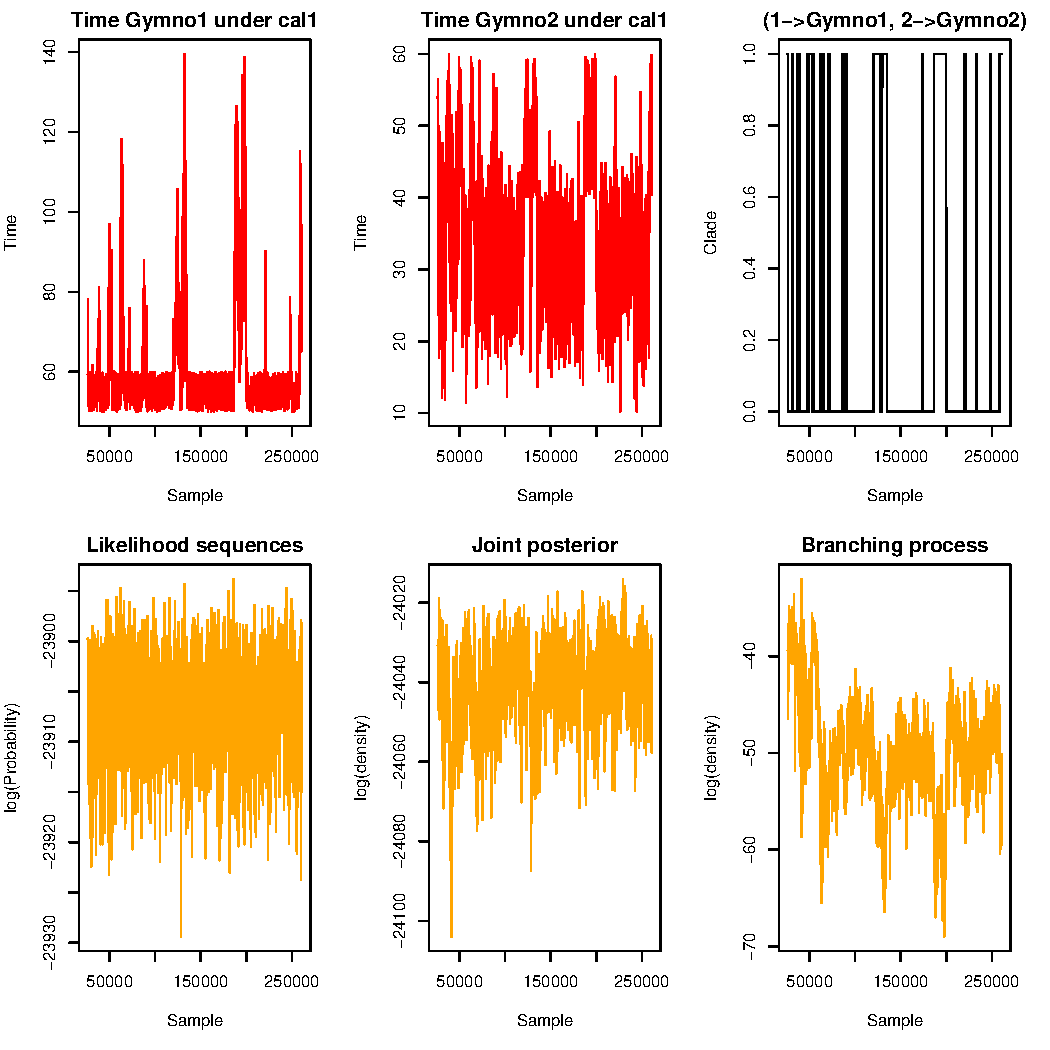
\includegraphics[width=13.8cm]{./fig/phytimetrace}
\end{center}
\caption{{\bf Traces from the statistics output file produced by PhyTime.}} 
\label{fig:phytimetrace}
\end{figure}

% Important  information is also  displayed on  the standard  output of  PhyTime (the  standard output
% generally corresponds to the terminal window from  which PhyTime was launched).  The first column of
% this output gives the current  generation, or run, of the chain. It starts at  1 and goes up to 1E+7
% by default.  The second column gives the time elapsed  in seconds since  the sampling  began. The
% third column  gives the  log likelihood  of the phylogenetic model (i.e., `Felsenstein's
% likelihood'). The  fourth column gives the logarithm of the joint prior  probability of substitution
% rates along  the tree and  node heights. The  fifth column gives the  current sampled value  of the
% EvolRate  parameter along with the  corresponding Effective Sample Size (ESS)  for this parameter.
% The sixth  column gives the tree height  and the  corresponding  ESS.  The seventh  column  gives
% the  value  of the  autocorrelation parameter followed by the  corresponding ESS. The eightth column
% gives the  values of the birth rate parameter that  governs the birth-rate model  of species
% divergence  dates.  The last column  of the standard  output gives  the minimum  of the  ESS  values
% taken  over the  whole set  of node  height estimates.  It provides useful information when one has
% to decide whether or not the sample size is large enough to draw  valid conclusion, i.e., decide
% whether the chain was  run for long enough (see Section \ref{sec:recomphytime} for more detail about
% adequate chain length).

% \subsubsection{ClockRate vs. EvolRate}

% The average rate of evolution along a branch  is broken into two components. One is called ClockRate
% and is  the same throughout  the tree. The  other is called EvolRate  and corresponds to  a weighted
% average of  branch-specific rates.  The  model of rate  evolution implemented in PhyTime  forces the
% branch-specific rate values to  be greater than one. As a consequence,  ClockRate is usually smaller
% EvolRate.

% In more mathematical terms, let $\mu$ be the value of ClockRate, $r_i$ be the value of the relative
% rate along branch $i$ and $\Delta_i$ the time elapsed along branch $i$. The value of EvolRate is
% then given by:
% \begin{eqnarray*}
% \mathrm{EvolRate} = \mu \frac{\sum_{i}^{2n-3} r_i \Delta_i}{\sum_{i}^{2n-3} \Delta_i}.
% \end{eqnarray*}  It is  clear from  this equation  that  multiplying each  $r_i$ by  a constant  and
% dividing $\mu$ by the same constant does not  change the value of EvolRate. The $r_i$s and $\mu$
% are then confounded,  or non-identifiable, and only  the value of EvolRate can  be estimated from
% the data.   {\color{red}{Please make sure  that you use  the value of  EvolRate rather than  that of
% ClockRate when referring to the estimate of the substitution rate}}.

% \subsubsection{Effective sample size}\label{sec:ess}

% The MCMC technique  generates samples from a  target distribution (in our case,  the joint posterior
% density  of  parameters).  Due  to  the  Markovian  nature of  the  method,  these samples  are  not
% independent.  The  ESS is the estimated  number of independent  measurements obtained from a  set of
% (usually dependent) measurements. It is calculated using the following formula:
% \begin{eqnarray*}
% \mathrm{ESS} = N\left(\frac{1-r}{1+r}\right),
% \end{eqnarray*}
% where  $N$  is the  length  of  the  chain  (i.e., the  `raw'  or `correlated' sample  size)  and $r$  is  the
% autocorrelation value, which is obtained using the following formula:
% \begin{eqnarray*}
% r = \frac{1}{(N-k)\sigma_x^2} \sum_{i=1}^{N-k} (X_i - \mu_x)(X_{i+k}-\mu_x),
% \end{eqnarray*} where $\mu_x$ and $\sigma_x$ are the mean and standard deviation of the $X_i$ values
% respectively and $k$ is the lag. The value of $r$ that is used in PhyTime corresponds to the case where $k=1$,
% which therefore gives a first order  approximation of the `average' autocorrelation value (i.e., the
% autocorrelation averaged over the set of possible values of the lag).


% \subsubsection{Prior distributions of model parameters}\label{sec:prior}

% Any Bayesian analysis requires  specifying a prior distribution of model  parameters. The outcome of
% the data analysis, i.e., the posterior distribution,  is influenced by the priors.  It is especially
% true if the signal conveyed  by the data is weak.  While some have  argued that the specification of
% priors relies more  on arbitrary decisions than sound scientific  reasoning, choosing relevant prior
% distributions  is in  fact fully  integrated in  the process  of building  model that  generates the
% observed data.  In particular, the problem of  estimating divergence times naturally lends itself to
% hierarchical Bayesian modelling.  Based on the hypothesis  that rates of evolution are conserved (to
% some extant)  throughout the  course of  evolution, the hierarchical  Bayesian approach  provides an
% adequate framework for inferring substitution rates  and divergence dates separately. Hence, in this
% situation, it makes good  sense to use what is known about a  relatively well-defined feature of the
% evolution of genetic sequences (the ``molecular  clock'' hypothesis combined to stochastic variations of
% rates across lineages) to build a prior distribution on rates along edges.




\subsubsection{Citing PhyTime}\label{sec:citephytime}

The ``default citation'' is:

\begin{itemize}
\item Guindon S. ``From trajectories to averages: an improved description of the heterogeneity of
substitution rates along lineages'', {\it Systematic Biology}, 2013. 62(1): 22-34.
\end{itemize}

If you are using mutliple calibrations on a given clade, please cite the following article:
\begin{itemize}
\item Guindon S. ``Accounting for calibration uncertainty: Bayesian molecular dating as a ``doubly intractable'' problem'', {\it Systematic Biology}, 2018. 67(4): 651-661.
\end{itemize}

An earlier article also describes some of the methods implemented in PhyTime:

\begin{itemize}
\item Guindon  S. ``Bayesian estimation of divergence  times from large data  sets'', {\it Molecular
    Biology and Evolution}, 2010,
27(8):1768:81.
\end{itemize}



\subsection{PhyloGeo}\index{PhyloGeo} PhyloGeo is  a program that implements the
competition-dispersal phylogeography model described in Ranjard, Welch, Paturel and Guindon
``Modelling competition  and  dispersal in a statistical phylogeographic framework''. Accepted for
publication in {\it Systematic Biology}.

It implements a  Markov Chain Monte Carlo  approach that samples from the  posterior distribution of
the three  parameters of  interest in this  model, namely  the competition intensity  $\lambda$, the
dispersal  bias parameter  $\sigma$ and  the overal  dispersal rate  $\tau$. The  data consist  in a
phylogeny with node heights proportional to their ages and geographical locations for evety taxon in
this tree. An important assumption of the model is that each node in the phylogeny corresponds to a
speciation {\em and} a dispersal event. As a consequence, this model does not authorize a given taxon to
occupy more than one locations. Note however that the converse is not true: a given location can be
occupied by several different taxa.

\subsubsection{Installing PhyloGeo}

Compiling PhyloGeo is straightforward on Unix-like  machines (i.e., linux and MacOS systems). PhyloGeo
is not readily available for Windows machines but  compilation should be easy on this system too. In
the `phyml' directory, where the `src/'  and `doc/' directories stand, enter the following commands:
{\setlength{\baselineskip}{0.5\baselineskip}
\begin{verbatim}
./configure --enable-geo;
make clean;
make;
\end{verbatim} } This set of commands generates  a binary file called \x{phylogeo} which can be found
  in the `src/' directory.

\subsubsection{Running PhyloGeo} PhyloGeo takes as input a rooted tree file in Newick format and a file
with geographical locations for all the tips of the phylogeny. Here is an example of valid tree and
the corresponding spatial locations just below:


\begin{scriptsize}
\begin{Verbatim}[frame=single, label=Valid PhyloGeo input tree, samepage=true, baselinestretch=0.5]
(((unicaA:1.30202,unicaB:1.30202):1.34596,(((nitidaC:0.94617,(nitidaA:0.31497,
nitidaB:0.31497):0.63120):0.18955,(((mauiensisA:0.00370,mauiensisB:0.00370):0.20068,
(pilimauiensisA:0.05151,pilimauiensisB:0.05151):0.15287):0.78769,(brunneaA:0.10582,
brunneaB:0.10582):0.88625):0.14365):0.80126,(((molokaiensisA:0.03728,
molokaiensisB:0.03728):0.71371,(deplanataA:0.01814,deplanataB:0.01814):0.73285):0.34764,
((parvulaA:0.20487,parvulaB:0.20487):0.40191,(kauaiensisA:0.24276,
kauaiensisB:0.24276):0.36401):0.49186):0.83835):0.71099):1.38043,
(nihoaA:0.05673,nihoaB:0.05673):3.97168);
\end{Verbatim}

\begin{Verbatim}[frame=single, label=Valid PhyloGeo spatial location file, samepage=true, baselinestretch=0.5]
nihoaA                  23.062222	161.926111
nihoaB                  23.062222	161.926111
kauaiensisA             22.0644445	159.5455555
kauaiensisB             22.0644445	159.5455555
unicaA                  21.436875	158.0524305
unicaB                  21.436875	158.0524305
parvulaA                21.436875	158.0524305
parvulaB                21.436875	158.0524305
molokaiensisA           20.90532	156.6499
molokaiensisB           20.90532	156.6499
deplanataA              20.90532	156.6499
deplanataB              20.90532	156.6499
brunneaA                20.90532	156.6499
brunneaB                20.90532	156.6499
mauiensisA              20.90532	156.6499
mauiensisB              20.90532	156.6499
pilimauiensisA          20.90532	156.6499
pilimauiensisB          20.90532	156.6499
nitidaA                 19.7362	        155.6069
nitidaB                 19.7362	        155.6069
nitidaC                 19.7362	        155.6069
\end{Verbatim}
\end{scriptsize}

In order to run PhyloGeo, enter the following command: \x{./phylogeo ./tree\_file
  ./spatial\_location\_file > phylogeo\_output}.
PhyloGeo will then print out the sampled values of the model parameters in the file
\x{phylogeo\_output}. This file can then be used to generate the marginal posterior densities of the
model parameters. In particular, evidence for competition corresponds to value of $\lambda$ smaller
than 1.0. Please see the original article for more information on how to interpret the model
parameters.

\subsubsection{Citing PhyloGeo}\label{sec:citephylogeo}

Ranjard, L., Welch D., Paturel M. and Guindon S. ``Modelling competition  and  dispersal in a
statistical phylogeographic framework''. 2014. Systematic Biology.



\subsection{PhyREX}\index{PhyREX} PhyREX is a program that implements the spatial
$\Lambda$-Fleming-Viot model
\cite{etheridge2008,berestycki2009,barton2010,barton2010b,veber2012,barton2013} or \sfv\ for short.
This model can be thought of as a structured-coalescent where space is considered as continuous
rather than organized into separate demes.
Under the \sfv\ model, the spatial distribution of individuals in a population is uniform and does
not change during the course of evolution, as opposed to other models such as the very popular
isolation by distance model proposed by Wright and Mal\'ecot. The \sfv\ model  does not
suffer from the ``pain in the torus'' \cite{felsenstein1975} and clumps of individuals with
increasing densities do not arise. Also, estimates of migration parameters are not sensitive to
variation in sampling intensities across regions, unlike ``mugration'' or ``discrete trait
analysis'' models \cite{lemey2009}.

PhyREX implements an original data augmentation technique embedded in a Bayesian sampler to
estimate two important biological parameters: the neighorhood size ($\mathcal{N}$) and the dispersal
intensity ($\sigma^2$). These two parameters are closely related to the effective size of the
population of interest per unit area since $\mathcal{N}$ is defined as follows: $\mathcal{N} := 4\pi
\rho_e \sigma^2$, where $\rho_e$ is the effective population density.

\subsubsection{Installing PhyREX}

Compiling PhyREX is straightforward on Unix-like  machines (i.e., linux and MacOS systems). PhyREX
is not readily available for Windows machines but  compilation should be easy on this system too. In
the `phyml' directory, where the `src/'  and `doc/' directories stand, enter the following commands:
{\setlength{\baselineskip}{0.5\baselineskip}
\begin{verbatim}
./configure --enable-phyrex;
make clean;
make;
\end{verbatim} } This set of commands generates  a binary file called \x{phyrex} which can be found
  in the `src/' directory.

\subsubsection{Running PhyREX}

Example input files for PhyREX can be found in the \x{examples/phyrex/} directory.
PhyREX takes as input a XML file (See Section \ref{sec:xmlio}), in a PhyML-compatible format. This
file defines the models and various parameter settings for conducting an analysis. We give more
information below about this file. The XML file gives the names of a sequence alignment file in the
standard PHYLIP (or NEXUS) format along with a file providing the spatial coordinates of the
corresponding sequences.  An example of the coordinates file is given
below:
\begin{Verbatim}[frame=single, label=Valid PhyREX spatial location file, samepage=true, baselinestretch=0.5]
# state.name lon lat
|SouthWest| 0 0
|NorthEast| 10 10 
levosl 5.082206 4.133893 
kmgcwv 5.914294 4.603446 
uhfwja 4.990937 4.445124 
ndmwkc 5.178017 4.442268 
jpadex 3.747484 4.571090 
lqcdcw 7.081925 5.133123 
wnsbtg 4.164588 4.720346 
ptwgnn 5.711159 4.462993 
jhqdsm 3.539525 4.537706 
vlnoes 4.613251 4.470530 
pfrnpk 4.117791 4.489819 
elwdvr 5.649958 4.824092 
lptxiv 4.563302 4.005124 
\end{Verbatim}
This first column in this  file gives the sequence names, the second is  the longitude and the third
column gives the latitude. The first row in this file gives the names of the columns. It starts with
the  `\#' character  signaling  a comment.  The  second and  third  rows define  the  limits of  the
population's habitat.  At the moment,  this habitat is  assumed to be  a rectangle. The  position in
space of that rectangle are determined by  the coordinates of the bottom-left corner (\x{|SouthWest|
0 0}) and the top-right one (\x{|NorthEast| 10  10}). The `\x{|}' characters help identify the terms
in the list of coordinate corresponding indeed to these two particular points and should thus not be
omitted. The  remaining row give  the coordinates of  each taxon. Every  taxon in the  sequence file
should also be listed in the coordinate file.

Below is an excerpt of a XML file that can be used as input to run a PhyREX analysis. The \sfv\
model parameters are estimated using a Bayesian sampler which hyperparameters (number of
samples, frequency at which samples are collected, length of the ``burnin'' phase, etc.) are set
through the corresponding XML attributes (see \ref{sec:phytimesettings}). PhyREX is similar to
PhyTime in the sense that substitution rates and times are separate parameters. The rates can
vary across lineages (using for instance a log-normal model) or not (strict clock). In case all
sequences were collected at (approximately) the same time, it is recommended to set the average
rate of evolution to a specific value (\x{<clockrate value="1E-4"/>}). Yet, with serially-sampled
data, the average rate of evolution can be estimated directly from the data and setting it to
a particular value is thus not mandatory. Finally, it is necessary to give information about the
time at which each sequence was collected. This is done through seeting appropriate calibration
constraints. From a technical perspective, these constraints apply to clades where each clade here
is a single tip.


\begin{Verbatim}[frame=single, label=Example (excerpt) of PhyREX XML file, samepage=true, baselinestretch=0.5,
  fontsize=\small, numbers=left]
  <phyrex run.id="example" output.file="out"
  mcmc.chain.len="1E+7"
  mcmc.sample.every="500"
  mcmc.print.every="100"
  mcmc.burnin="10000"
  mutmap="no">
  
  <!-- ``Standard'' stuff goes here, i.e., <topology>, -->
  <!-- <partitionelem>, etc -->
  
  <!-- Model of rate variation across lineages -->
  <lineagerates model="lognormal"/>
  
  <!-- Set the average (clock) rate of substitution -->
  <!-- to a fixed value (optional) -->
  <clockrate value="1E-4"/>

  <-- File where 2-D spatial coordinates are found --> 
  <coordinates id="coordinates" file.name="./usa_coord.txt"/>

  <!-- Set the date for each tip. Useful in serial sample -->
  <!-- analysis -->
  <clade id="clad1">
  <taxon value="CY130177|South_Carolina|12_13|H1N1"/>
  </clade>

  <!-- Clade 1 (made of a single sequence) has time set to 0 -->
  <calibration id="cal1">
    <lower>0</lower>
    <upper>0</upper>
    <appliesto clade.id="clad1"/>
  </calibration>

  
  <clade id="clad2">
  <taxon value="KF647978|Idaho|12_13|H1N1"/>
  </clade>
  
  <!-- Clade 2 has time set to 10 -->
  <calibration id="cal2">
    <lower>10</lower>
    <upper>10</upper>
    <appliesto clade.id="clad2"/>
  </calibration>
  
  <!-- More calibration info goes here. At least, one -->
  <!-- calibrated clade per tip. -->  
  
\end{Verbatim}

PhyREX generates correlated samples from the posterior distribution of the \sfv\ model
parameters. The estimated distributions and related summary statistics can be monitored during the
analysis using the MCMC vizualization software Icylog. Figure \ref{fig:phyrextrace} shows the traces
for two parameters after about an hour of calculation on the example data set (36 taxa, 50
geographic locations). Most of the names of the sampled parameters are self-explanatory but some of
them (listed below) need explanations:
\begin{itemize}
\item \texttt{lnP} : log-posterior.
\item \texttt{alnL} : logarithm of the probability of the sequence alignment given the current tree.
\item \texttt{glnL} : logarithm of the probability of the current tree and location data. 
\item \texttt{clock} : substitution rate
\item \texttt{lbda} : value of $\lambda$, the rate at which REX events take place in the \sfv~model.
\item \texttt{mu} : value of $\mu$, the term governing the probability for the lineage to be hit by
  a REX event.
\item \texttt{rad} : value of the parameter $\theta$, i.e., the radius parameter in the \sfv~model.
\item \texttt{neigh} : neighborhood size (equal to $2/\mu$ under the \sfv~model).
\item \texttt{rhoe} : effective population density.
\item \texttt{sigsq} : $\sigma^2 := 4\theta^4\lambda \pi \mu /s$ where $s$ is the surface of the habitat.
\item \texttt{sigsqobs} : mean, taken over the (most recent) tips, of one half (in a two-dimensional space) times the Euclidean distance
  covered in one unit of time, squared.
\item \texttt{dispdist} : mean, taken over the (most recent) tips, of the Haversine distance
  covered in one unit of time.
\item \texttt{nInt} : number of REX events.
\item \texttt{nCoal} : number of coalescent events.
\item \texttt{nHit} : number of REX events where a single lineage was hit.
\item \texttt{rootTime} : time at the root node.
\item \texttt{rootLon} : longitude of the root node location.
\item \texttt{rootLat} : latitude of the root node location.
\end{itemize}
If you
are unsure about the precise definition of one of these parameters or have any questions regarding
how to interpret the results returned by PhyREX, please do not hesitate to contact me (\url{guindon@lirmm.fr}).

\begin{figure}
\begin{center}
  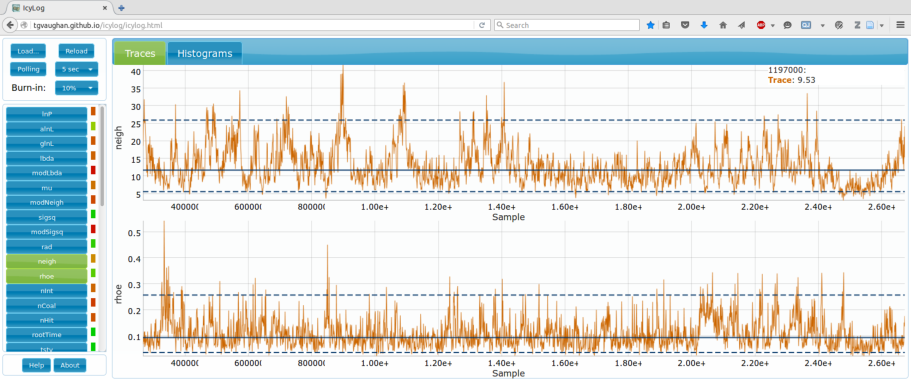
\includegraphics[width=13.8cm]{./fig/phyrexlog}
\end{center}
\caption{{\bf Statistics file generated by PhyREX and loaded on Icylog
    (\url{http://tgvaughan.github.io/icylog/icylog.html}).} The traces for the neighborhood size
  (top) and
the dispersal intensity (bottom) are shown here.} 
\label{fig:phyrextrace}
\end{figure}

\subsubsection{Citing PhyREX}

The ``default citation'' is:

\begin{itemize}
\item Guindon S.,  H Guo, D Welch. ``Demographic inference under the coalescent in a spatial
  continuum'', {\it Theoretical Population Biology}, 2016, 111:43-50.
\end{itemize}

\section{Recommendations on program usage}\label{sec:progusage}

\subsection{PhyML}

The choice of the  tree searching algorithm among those provided by PhyML  is generally a tough one.
The  fastest option  relies  on local  and simultaneous  modifications  of the  phylogeny using  NNI
moves. More  thorough explorations of  the space  of topologies are  also available through  the SPR
options.  As these  two classes of tree topology moves involve  different computational burdens, it
is important to determine which option is the most suitable for the type of data set or analysis one
wants to perform. Below is a list of recommendations for typical phylogenetic analyses.

\begin{enumerate}
\item {\em Single data set, unlimited computing time.} The best option here is probably to use a SPR
search (i.e., straight SPR of best of SPR and NNI).  If the focus is on estimating the relationships
between species,  it is a good  idea to use  more than one starting  tree to decrease the  chance of
getting stuck  in a  local maximum of  the likelihood  function.  Using NNIs  is appropriate  if the
analysis does not mainly focus on  estimating the evolutionary relationships between species (e.g. a
tree is needed to  estimate the parameters of codon-based models later  on).  Branch supports can be
estimated using bootstrap and approximate likelihood ratios.

\item {\em  Single data set, restricted  computing time.}  The  three tree searching options  can be
used depending on  the computing time available and the  size of the data set.   For small data sets
(i.e., $<$ 50 sequences),  NNI will generally perform well provided that  the phylogenetic signal is
strong.  It  is relevant  to estimate a  first tree  using NNI moves  and examine  the reconstructed
phylogeny in order to have a rough idea  of the strength of the phylogenetic signal (the presence of
small internal  branch lengths  is generally  considered as a  sign of  a weak  phylogenetic signal,
specially when  sequences are  short).  For larger  data sets  ($>$ 50 sequences),  a SPR  search is
recommended if there  are good evidence of  a lack of phylogenetic signal.   Bootstrap analysis will
generally  involve  large  computational  burdens.   Estimating branch  supports  using  approximate
likelihood ratios therefore provides an interesting alternative here.

\item {\em  Multiple data  sets, unlimited computing  time.} Comparative genomic  analyses sometimes
rely on building phylogenies from the analysis of  a large number of gene families.  Here again, the
NNI option is the most  relevant if the focus is not on recovering the  most accurate picture of the
evolutionary relationships  between species.   Slower SPR-based heuristics  should be used  when the
topology of the tree is an important parameter of the analysis (e.g., identification of horizontally
transferred genes using phylogenetic tree comparisons).   Internal branch support is generally not a
crucial parameter of the multiple data  set analyses. Using approximate likelihood ratio is probably
the best choice here.

\item {\em Multiple data sets, limited computing time.}  The large amount of data to be processed in
a  limited time  generally  requires  the use  of  the fastest  tree  searching  and branch  support
estimation methods Hence,  NNI and approximate likelihood ratios rather  than SPR and non-parametric
bootstrap are generally the most appropriate here.
\end{enumerate}

Another important  point is the  choice of the  substitution model. While default  options generally
provide acceptable results, it is often warranted to perform a pre-analysis in order to identify the
best-fit substitution model.  This pre-analysis can be done using popular software such as Modeltest
\cite{posada98} or ProtTest  \cite{abascal05} for instance.  These programs  generally recommend the
use of a discrete gamma distribution to model the substitution process as variability of rates among
sites is a common  feature of molecular evolution.  The choice of the number  of rate classes to use
for this  distribution is  also an important  one. While the  default is  set to four  categories in
PhyML, it is  recommended to use larger number  of classes if possible in order  to best approximate
the  patterns of rate  variation across  sites \cite{galtier04}.   Note however  that run  times are
directly proportional to  the number of classes  of the discrete gamma distribution.   Here again, a
pre-analysis with the  simplest model should help the  user to determine the number  of rate classes
that represents the best trade-off between computing time and fit of the model to the data.


\subsection{PhyTime}\label{sec:recomphytime}

Analysing a data set using PhyTime should  involve three steps based on the following questions: (1)
do the priors seem to be adequate (2) can I use the fast approximation of the likelihood and (3) how
long shall I run the program for? I explain below how to provide answers to these questions.

\begin{itemize}
\item {\em  Are the priors adequate?} Bayesian  analysis relies on  specifiying the joint
prior density  of model parameters.  In  the case of  node age estimation, these  priors essentially
describe how rates of substitution vary across lineages and the probabilistic distribution that node
ages have when  ignoring the information provided  by the genetic sequences. These  priors vary from
tree to tree. It is therefore essential to  check the adequacy of priors for each user-defined input
tree. In order to do so, PhyTime needs to be run with the \x{--no\_data} option. When this option is
required, the  sequence data provided  as input will  be ignored and the  rest of the  analysis will
proceed  normally. The  prior distribution  of  model parameters,  essentially edge  rates and  node
heights, can then be  checked using the program Tracer as one would  do for the standard `posterior'
analysis.

\item {\em  Can I use the  fast approximation to the  likelihood?} The suface  of the log-likelihood
function can  be approximated using  a multivariate normal  density.  This technique is  saving very
substantial amounts  of computation  time. However, like  most approximations, there  are situations
where it does not provide a good fit to the actual function. This usually happens when the phylogeny
displays  a lot  of short  branches, i.e.,  the  signal conveyed  by the  sequences is  weak. It  is
therefore important to first check whether  using the approximate likelihood is reasonable. In order
to do  so, it is  recommended to first  run the program without  the approximation, i.e.,  using the
default settings. Once  the minimum value of the ESS  of node ages (the last column  on the right of
the  standard output)  has reached  40-50, open  the \x{phytime.XXXX}  output file  with  Tracer and
examine the correlation  between the exact and approximate likelihood values.  If the correlation is
deemed to be good enough, PhyTime can be re-run using the \x{--fast\_lk} option, which uses the fast
normal approximation to the likelihood function.



% Figure \ref{fig:approxbad} gives an example where  the correlation is too weak and the approximation
% of  the  likelihood  should be  avoided.  Figure  \ref{fig:approxbad}  gives  an example  where  the
% approximation  is  good enough.   The  current  execution of  PhyTime  can  be  terminated and  then
% re-launched using the \x{--fast\_lk} option.

% \begin{figure}
% \begin{center}
% \resizebox{14cm}{8cm}{\includegraphics{./fig/approx_bad.eps}}
% \caption{{\bf Exact vs. approximate likelihoods.} The correlation between the normally approximated
%   (Y-axis) and the exact (X-axis) likelihoods is weak here. The exact likelihood should be used (option \x{fastlk=no}).}
% \label{fig:approxbad}
% \end{center}
% \end{figure}


% \begin{figure}
% \begin{center}
% \resizebox{14cm}{8cm}{\includegraphics{./fig/approx_good.eps}}
% \caption{{\bf Exact vs. approximate likelihoods.} The correlation between the normally approximated
%   (Y-axis) and the exact (X-axis) likelihoods is good. The approximation of the  likelihood can be used (option \x{fastlk=yes}).}
% \label{fig:approxgood}
% \end{center}
% \end{figure}

\item {\em How  long shall I run the program  for?} PhyTime should be run long  enough such that the
ESS of  each parameter  is `large enough'.  The last column  on the  right handside of  the standard
output gives the minimum ESS across all internal  node heights. It is recommended to run the program
so that this number reaches at least 100.

\end{itemize}


\section{Frequently asked questions}

\begin{enumerate}
\item {\it PhyML crashes before reading the sequences. What's wrong ?}\\
\begin{itemize}
\item The format of your sequence file is not recognized by PhyML. See Section \ref{sec:input_output}
\item The carriage return characters in your sequence files are not recognized by PhyML. You must
  make sure that your sequence file is a plain text file, with standard carriage return characters (i.e.,
  corresponding to ``$\backslash$\x{n}'', or ``$\backslash$\x{r}'')
\end{itemize}
\item {\it The program crashes after reading the sequences. What's wrong ?}\\
\begin{itemize}
\item You analyse protein sequences and did not enter the \x{-d aa} option in the command-line.
\item The format of your sequence file is not recognized by PhyML. See Section \ref{sec:input_output}
\end{itemize}
\item {\it Does PhyML handle outgroup sequences ?}\\
\begin{itemize}
\item Yes, it does. Outgroup taxa are identified by adding the `*' sign at the end of each
  corresponding sequence name (see Section \ref{sec:outgroupspecify})
\end{itemize}
\item {\it Does PhyML estimate clock-constrained trees ?}\\
\begin{itemize}
\item No, the PhyML program does not estimate clock-contrained trees. One can however use the
  program PhyTime to perform such analysis but the tree topology will not be estimated.
\end{itemize}
\item {\it Can PhyML analyse partitioned data, such as multiple gene sequences ?}\\
\begin{itemize}
\item We are currently  working on this topic.  Future releases of  the program will provide options
to estimate  trees from phylogenomic data sets,  with the opportunity to  use different substitution
models on  the different data partitions (e.g.,  different genes). PhyML will  also include specific
algorithms to search the space of tree topologies for this type of data.
\end{itemize}
\end{enumerate}



\section{Acknowledgements}
The development of PhyML since 2000 has been supported by the Centre National de la Recherche
Scientifique (CNRS) and the Minist\`ere de l'\'Education Nationale.

\bibliographystyle{./naturemag}
\bibliography{./ref.bib}

\printindex
\end{document}

